% Final BTech Major Project Report.
% Build: see report/BUILD.md  (tectonic final_report.tex, run inside report/)
% Every number in this report traces to a file named in the "Sources" notes
% (results/, pilot_b/, pilot_original/, phase2/, research/, docs/DECISIONS.md,
% paper/latex/main.tex). Red bracketed text marks items the student must fill.
\documentclass[12pt,a4paper,oneside]{report}

\usepackage{fontspec}
\setmainfont{texgyretermes}[Extension=.otf,UprightFont=*-regular,BoldFont=*-bold,ItalicFont=*-italic,BoldItalicFont=*-bolditalic]
\setmonofont{lmmono10-regular}[Extension=.otf,Scale=0.95,BoldFont=lmmonolt10-bold,ItalicFont=lmmono10-italic,BoldItalicFont=lmmonolt10-boldoblique]
\usepackage[a4paper,left=3.5cm,right=2.5cm,top=2.5cm,bottom=2.5cm]{geometry}
\usepackage{setspace}
\onehalfspacing
\usepackage{graphicx}
\usepackage{booktabs}
\usepackage{tabularx}
\usepackage{longtable}
\usepackage{array}
\usepackage{multirow}
\usepackage{xcolor}
\usepackage{enumitem}
\usepackage{caption}
\captionsetup{font=small,labelfont=bf}
\usepackage{tikz}
\usetikzlibrary{arrows.meta,positioning,shapes.geometric,fit}
\usepackage{tfrupee}
\usepackage[numbers,sort&compress]{natbib}
\usepackage{titlesec}
\titleformat{\chapter}[display]{\normalfont\Large\bfseries}{\chaptertitlename\ \thechapter}{12pt}{\LARGE}
\titlespacing*{\chapter}{0pt}{-20pt}{24pt}
\usepackage{fancyhdr}
\pagestyle{fancy}
\fancyhf{}
\fancyhead[R]{\small\nouppercase{\leftmark}}
\fancyfoot[C]{\thepage}
\renewcommand{\headrulewidth}{0.4pt}
\fancypagestyle{plain}{\fancyhf{}\fancyfoot[C]{\thepage}\renewcommand{\headrulewidth}{0pt}}
\usepackage{xurl}
\usepackage[hidelinks]{hyperref}
\usepackage{seqsplit}
\usepackage{makecell}
% Allow line breaks after underscores and slashes in identifiers.
\let\oldunderscore\_
\renewcommand{\_}{\oldunderscore\allowbreak}
\setlength{\emergencystretch}{3em}
\newcommand{\hash}[1]{\texttt{\seqsplit{#1}}}

% Visible placeholders for details only the student can supply.
\newcommand{\placeholder}[1]{\textcolor{red}{\textbf{[}\textit{#1}\textbf{]}}}
\newcommand{\rs}{\rupee}
\newcommand{\form}[1]{\textbf{#1}}
\newcommand{\evid}[1]{\par\noindent\fbox{\parbox{\dimexpr\linewidth-2\fboxsep-2\fboxrule}{\small\textbf{Evidence label:} #1}}\par\medskip}
\newcolumntype{L}{>{\raggedright\arraybackslash}X}

\begin{document}

%======================================================================
% TITLE PAGE
%======================================================================
\begin{titlepage}\singlespacing
\begin{center}
\vspace*{-0.5cm}
{\LARGE\bfseries Romanized Hindi Is Harder Than Hinglish:\\[4pt] A Scoring-Aware Audit of Small LLMs on\\[4pt] Mathematical Word Problems\par}
\vspace{0.8cm}
{\large Major Project Report\par}
\vspace{0.3cm}
{\large submitted in partial fulfilment of the requirements for the award of the degree of\par}
\vspace{0.3cm}
{\Large\bfseries Bachelor of Technology\par}
\vspace{0.2cm}
{\large in\par}
\vspace{0.2cm}
{\large \placeholder{Department / Branch name}\par}
\vspace{0.8cm}
{\large Submitted by\par}
\vspace{0.3cm}
{\large \placeholder{Student Name 1} \enspace (\placeholder{Roll No. 1})\par}
{\large \placeholder{Student Name 2, if any} \enspace (\placeholder{Roll No. 2})\par}
\vspace{0.8cm}
{\large Under the supervision of\par}
\vspace{0.3cm}
{\large \placeholder{Supervisor Name}\par}
{\large \placeholder{Designation, Department}\par}
\vfill
\placeholder{DTU logo (optional)}\\[0.6cm]
{\large\bfseries \placeholder{Department name}\\ Delhi Technological University\par}
{\large (Formerly Delhi College of Engineering)\\ Bawana Road, Delhi -- 110042\par}
\vspace{0.5cm}
{\large November 2026\par}
\end{center}
\end{titlepage}

\pagenumbering{roman}
\setcounter{page}{2}

%======================================================================
% CERTIFICATE
%======================================================================
\chapter*{Certificate}
\addcontentsline{toc}{chapter}{Certificate}
\thispagestyle{plain}
\markboth{Certificate}{}

I hereby certify that the project report entitled \textbf{``Romanized Hindi Is Harder Than Hinglish: A Scoring-Aware Audit of Small LLMs on Mathematical Word Problems''}, submitted by \placeholder{Student Name(s)} (\placeholder{Roll No(s).}) to the \placeholder{Department name}, Delhi Technological University, in partial fulfilment of the requirements for the award of the degree of Bachelor of Technology, is a record of the project work carried out by the student(s) under my supervision. To the best of my knowledge, this work has not been submitted in part or in full for any degree or diploma at this university or elsewhere.

\vspace{3cm}
\noindent
\begin{tabular}{@{}l@{\hspace{5cm}}l@{}}
Place: Delhi & \placeholder{Supervisor signature}\\
Date: \placeholder{Date} & \placeholder{Supervisor Name}\\
 & \placeholder{Designation}\\
 & \placeholder{Department}, Delhi Technological University\\
\end{tabular}

%======================================================================
% DECLARATION
%======================================================================
\chapter*{Candidate's Declaration}
\addcontentsline{toc}{chapter}{Candidate's Declaration}
\thispagestyle{plain}
\markboth{Candidate's Declaration}{}

I/We, \placeholder{Student Name(s)} (\placeholder{Roll No(s).}), students of B.Tech.\ (\placeholder{Branch}), hereby declare that the project report entitled \textbf{``Romanized Hindi Is Harder Than Hinglish: A Scoring-Aware Audit of Small LLMs on Mathematical Word Problems''}, submitted to the \placeholder{Department name}, Delhi Technological University, in partial fulfilment of the requirements for the award of the degree of Bachelor of Technology, is original and has not been submitted, in part or in full, for any other degree or diploma.

The use of AI assistants in the project is disclosed in full in Section~\ref{sec:aidisclosure}. Human reviewers made every dataset acceptance decision, and I/we take responsibility for the content of this report.

\vspace{3cm}
\noindent
\begin{tabular}{@{}l@{\hspace{5cm}}l@{}}
Place: Delhi & \placeholder{Student signature(s)}\\
Date: \placeholder{Date} & \placeholder{Student Name(s), Roll No(s).}\\
\end{tabular}

%======================================================================
% ACKNOWLEDGEMENTS
%======================================================================
\chapter*{Acknowledgements}
\addcontentsline{toc}{chapter}{Acknowledgements}
\thispagestyle{plain}
\markboth{Acknowledgements}{}

\placeholder{Thank the supervisor by name and designation.}

\placeholder{Thank the Head of Department and the department by name.}

I/We thank the bilingual team members and volunteers who solved, reviewed and repaired the problem renderings, and the adjudicator who confirmed the reference answers for the original pilot. All reviewers consented to the release of the reviewed data under CC BY 4.0. In keeping with their stated preferences, reviewers are not named here; the adjudicator declined credit.
\placeholder{Optionally add reviewers who have asked to be credited, by name, only with their written agreement.}

\placeholder{Add any other acknowledgements (family, friends, compute providers).}

%======================================================================
% ABSTRACT
%======================================================================
\chapter*{Abstract}
\addcontentsline{toc}{chapter}{Abstract}
\thispagestyle{plain}
\markboth{Abstract}{}

Many Indian users ask mathematical questions in Hinglish, a mix of Hindi and English usually written in Roman script. This project asks whether the language form of an otherwise identical word problem changes whether a small open large language model (LLM) solves it. Each problem is rendered in three matched forms: English (\form{E}), Romanized Hindi (\form{R}) and Roman-script Hinglish (\form{C}). Gold answers are computed in code, renderings are solved blind by two LLMs, and bilingual humans review the families. Models are evaluated unchanged (4-bit NF4 on a Colab T4) with one fixed English instruction, greedy decoding and a frozen strict scorer, under analysis plans written before any output on each cohort.

On 36 permanently excluded development fixtures, a plausible answer-format instruction made 10/36 Qwen3-4B outputs fail strict scoring and pushed 8/12 R explanations into Devanagari. After one disclosed prompt revision both counts were zero, and a seven-model screen showed that format compliance is strongly model-specific; three models passed a pre-declared inclusion rule.

In two separately reviewed, pre-registered cohorts, which are never pooled, R is the lowest-scoring form for all three backbones. On the primary 70-family Pilot-B cohort, Qwen3-4B scores 94.3/85.7/94.3\% on E/R/C, Qwen3-8B 98.6/91.4/98.6\% and Llama-3.2-3B 94.3/57.1/70.0\%. A 24-family cohort from the original pilot shows the same direction, with Qwen near ceiling. Both Qwen models have equal observed aggregate accuracy on E and C in both cohorts, which is not an equivalence result. The R errors are not concentrated in items that contain Hindi operation words. An audit of the primary model's outputs places most substantive errors in R and shows English-explanation compliance falling from 70/70 (E) to 53/70 (R).

The ordering R~$<$~C is not new: prior work reports it on translated GSM8K items. This project contributes newly drafted, human-reviewed triplets, a scoring-aware frozen protocol, two separately reviewed cohorts and a reproducible pipeline. It also prepares 300 frozen families for a planned E+E/E+R/E+C fine-tuning study, to be carried out by May 2027.

\vspace{0.5cm}
\noindent\textbf{Keywords:} Hinglish, Romanized Hindi, code-mixing, mathematical reasoning, LLM evaluation, answer extraction, pre-registration.

%======================================================================
\tableofcontents
\listoffigures
\listoftables

%======================================================================
% ABBREVIATIONS
%======================================================================
\chapter*{List of Abbreviations}
\addcontentsline{toc}{chapter}{List of Abbreviations}
\thispagestyle{plain}
\markboth{List of Abbreviations}{}

\begin{longtable}{@{}p{3.2cm}p{10.5cm}@{}}
\toprule
\textbf{Term} & \textbf{Meaning}\\
\midrule
\endhead
A01 & Pseudonym of the adjudicator of the original pilot review\\
ARR & ACL Rolling Review\\
BBPE & Byte-level byte-pair encoding\\
\form{C} & Roman-script Hinglish (code-mixed) rendering\\
CC BY 4.0 & Creative Commons Attribution 4.0 licence\\
CI & Confidence interval\\
CMI & Code-Mixing Index\\
CSV & Comma-separated values\\
D001--D038 & Entries in the project decision log (\texttt{docs/DECISIONS.md})\\
DEV & Phase-2 development split\\
\form{E} & English rendering\\
EACL & Conference of the European Chapter of the ACL\\
FINAL\_TEST & Phase-2 held-out test split, untouched until the confirmatory evaluation\\
FMT2 & The 12 excluded format-test fixture families (36 prompts)\\
FP16 & 16-bit floating point\\
GPU & Graphics processing unit\\
GSM8K & Grade School Math 8K benchmark\\
JSON / JSONL & JavaScript Object Notation / one JSON object per line\\
LLM & Large language model\\
LoRA / QLoRA & Low-rank adaptation / quantized LoRA\\
MGSM & Multilingual Grade School Math\\
MIT & The MIT software licence\\
NF4 & 4-bit NormalFloat quantization\\
pp & Percentage points\\
\form{R} & Romanized Hindi rendering\\
R01, R02 & Pseudonyms of the two reviewers of the original pilot\\
RQ & Research question\\
SDPA & Scaled dot-product attention\\
SHA-256 & Secure Hash Algorithm, 256-bit digest\\
SRW & Student Research Workshop\\
T4 & NVIDIA Tesla T4 GPU (Google Colab)\\
TRAIN & Phase-2 training split\\
\bottomrule
\end{longtable}

\cleardoublepage
\pagenumbering{arabic}

%======================================================================
\chapter{Introduction}
\label{ch:intro}
%======================================================================

\section{Motivation}

A model that answers ``How many marbles does Aman have?'' may fail on \emph{Aman ke paas kitne kanche hain?} although the mathematics is identical. Hundreds of millions of people write Hindi in the Latin alphabet in messages, search queries and chat, often mixing in English words. If an assistant becomes less reliable when a student asks the same question in this everyday form, the reliability gap falls on exactly the users that such assistants are meant to reach.

Measuring this gap is harder than it looks. If accuracy drops on a Hinglish question, the cause could be Hindi vocabulary, Roman-script spelling, the mixing of languages within a sentence, a harder or ambiguous wording, or the evaluation protocol itself: a correct answer written in an unexpected format can be scored as wrong. Comparing unrelated English and Hinglish questions cannot separate these causes. This project therefore holds the mathematics fixed and varies only the language form.

\section{The E/R/C problem}

Each mathematical \emph{family} is one problem rendered three times:
\begin{itemize}[nosep]
\item \form{E}: English;
\item \form{R}: Hindi phrasing written in Roman script, with a short borrowing list for numbers, units and established loanwords;
\item \form{C}: Roman-script Hindi with English lexical material beyond that list (Hinglish).
\end{itemize}
A model sees each rendering in a fresh context, with one fixed English instruction, and is scored by one frozen scorer. Because the three renderings share their mathematics and gold answer, differences in correctness across E, R and C are differences in how the model handles the language form, conditional on the renderings being equivalent and natural. Ensuring that condition is the job of the review process described in Chapter~\ref{ch:method}.

\section{Research questions}

The project has two phases. The phase reported here answers the first question; the other two belong to the planned training study (Chapter~\ref{ch:conclusion}).

\begin{description}[leftmargin=1.2cm,style=nextline]
\item[RQ1 (this phase)] How does an unchanged model's correctness differ across mathematically equivalent E, R and C prompts?
\item[RQ2 (training study)] Does E+C fine-tuning improve held-out C accuracy over matched E+R fine-tuning?
\item[RQ3 (training study)] Do any gains transfer to unseen phrasing and spellings, and what happens to English accuracy?
\end{description}

\section{Contributions}

The ordering found here, with Romanized Hindi below Hinglish, is not a new discovery. CodeMixTax~\citep{sthanika-2026-codemix} aligns the same 955 GSM8K questions across five forms and already reports Romanized Hindi below Romanized Hinglish; this is direct prior evidence for the main result. \citet{peter-etal-2026-mind} show that translation errors and answer extraction can distort multilingual math gaps. Building on that evidence, this project provides a reproducible, scoring-aware audit of small open LLMs. Its contributions are:
\begin{enumerate}[nosep]
\item \textbf{New triplets.} The 370 frozen families were drafted rather than derived from GSM8K and are written in natural Roman spelling rather than scheme transliteration. Every family has code-computed gold and blind dual-model verification, and all evaluated cohorts were human-reviewed.
\item \textbf{A scoring-aware frozen protocol.} On excluded fixtures, a plausible final-answer instruction caused form-dependent scoring failures and language drift. One disclosed revision removed both, and a seven-model compliance screen with a pre-declared rule preceded model admission.
\item \textbf{Two separately reviewed, pre-registered cohorts}, analysed and reported separately, whose direction is consistent: R is the lowest-scoring form for all three backbones.
\item \textbf{A negative result on a plausible mechanism.} The development data suggested that Hindi operation words (\emph{bhaag}, \emph{bhinn}) cause R errors. A balanced keep/switch design tested this, and the R errors were not concentrated in such items.
\item \textbf{A reproducible system}: self-contained Colab notebooks with an append-only journal and resume, a frozen scorer plus a pre-registered secondary endpoint, checksummed result exports, an independent table builder, a blind-solver toolkit and an authoring kit, with 161 passing software tests.
\end{enumerate}

\section{Report outline}

Chapter~\ref{ch:lit} reviews related work. Chapter~\ref{ch:method} defines the forms, describes how the datasets were drafted, verified and reviewed, and lists the frozen datasets. Chapter~\ref{ch:system} describes the evaluation software and its testing. Chapter~\ref{ch:dev} reports the development findings on excluded fixtures that shaped the protocol. Chapter~\ref{ch:results} reports the results for both cohorts and the output audit. Chapter~\ref{ch:discussion} discusses them, Chapter~\ref{ch:limits} sets out limitations and ethics, and Chapter~\ref{ch:conclusion} concludes and describes the training study planned for the rest of the project. Appendices give the frozen prompt, dataset hashes, the decision log, the review forms and reproduction instructions.

Throughout, every result carries an \emph{evidence label}: software verification, development evidence on excluded fixtures, or a cohort result. Cohorts are never pooled.

%======================================================================
\chapter{Literature Review}
\label{ch:lit}
%======================================================================

This chapter places the project among prior work on multilingual mathematical reasoning, code-mixed and Romanized evaluation, and the measurement problems that affect both. The citations come from a bibliography whose entries were each checked against a primary source (ACL Anthology, arXiv, DOI records or publisher pages). A bounded novelty refresh on 26 October 2026 inspected fifteen recent works; it is a targeted primary-source audit, not an exhaustive review.

\section{Mathematical word problems and multilingual reasoning}

GSM8K~\citep{cobbe-etal-2021-gsm8k} is the standard English grade-school benchmark: 7,473 training and 1,319 test problems, each with a numeric answer. MGSM~\citep{shi-etal-2023-mgsm} translates 250 GSM8K test problems into ten languages by hand and shows that chain-of-thought reasoning transfers across languages, but it contains no Hindi.

For Hindi, GSM8K-Hi~\citep{kamath-etal-2025-benchmarking} is a machine translation of the GSM8K test set into Devanagari, reviewed and corrected by humans. HAWP~\citep{sharma-etal-2022-hawp} contains 2,336 Hindi arithmetic word problems with equation annotations; its authors document wrong word senses and translation errors during construction. \citet{anand-etal-2025-multilingual} fine-tune open models on Hindi and English mathematics, explicitly excluding Romanized Hindi. Several studies train for multilingual mathematical reasoning: mCoT~\citep{lai-nissim-2024-mcot} targets reasoning consistency across languages, MathOctopus~\citep{chen-etal-2024-breaking} studies multilingual instruction data, and XCOT~\citep{chai-etal-2025-xcot} uses cross-lingual instruction tuning while keeping English responses for translated queries. None of these isolates the Roman-script forms that Indian users commonly type.

\section{Code-mixed and Romanized evaluation}

\paragraph{CodeMixTax.} The closest prior work is the CodeMixTax report~\citep{sthanika-2026-codemix}. It aligns the same 955 GSM8K questions (and MMLU items) across five forms (English, Devanagari Hindi, mixed-script Hinglish, Romanized Hinglish and Romanized Hindi) and evaluates 16 models. Romanized Hindi falls below Romanized Hinglish; for example, it reports E/Romanized-Hinglish/Romanized-Hindi maths accuracy of 90.26/66.18/40.63 for Gemma-3-4B. Its Romanized forms come from deterministic scheme-style romanization of machine-translated Hindi, and the report acknowledges semantic translation drift. It is an author research report, not a peer-reviewed paper. This project builds directly on it: the ordering is the same, while the items, spelling style, review and scoring protocol differ.

\paragraph{CodeMixBench and Indi-RomCoM.} CodeMixBench~\citep{yang-chai-2025-codemixbench} evaluates code-mixing across 18 languages and eight tasks. Its Hindi--English GSM8K variant mixes Devanagari Hindi with Latin-script English, so it is not a Roman-script comparison, and tested models score lower on it than on English. Indi-RomCoM~\citep{das-etal-2026-indiromcom} (a preprint) varies the intensity of Romanized code-mixing (25/50/75\%) for four Indic languages on tasks including GSM8K, but has no separate monolingual Romanized-language condition, and asks for output in the input language and script.

\paragraph{Romanized input elsewhere.} Sarvam-M~\citep{sarvam-2025-sarvamm}, an author technical report, shows GSM8K accuracy falling from native-script to Romanized Indic input. Romanized input also hurts LLM triage of real health messages in Indian languages~\citep{khullar-etal-2026-script}. These results support the existence of a script or romanization penalty but do not include a matched code-mixed condition.

\section{Measurement: translation errors and answer extraction}

\citet{peter-etal-2026-mind} audit MGSM and show that translation errors, ambiguous source questions and answer-extraction details (for example, numerals in another script) can create or remove apparent language gaps; after repairs, many gaps shrink. This is the methodological predecessor of the present project's scoring-aware design. It does not license changing a frozen scorer after seeing results; it motivates checking the scorer on excluded data \emph{before} the evaluation, which is what Chapter~\ref{ch:dev} reports.

\section{Operation cues, spelling and tokenization}

Mathematical solvers can exploit shallow cues: SVAMP~\citep{patel-etal-2021-nlp} showed that English word-problem solvers performed well even without the question text, and GSM-Symbolic~\citep{mirzadeh-etal-2025-gsmsymbolic} shows that LLMs turn irrelevant phrases into operations. This motivates the operation-word hypothesis tested here: that Hindi words such as \emph{bhinn} (``fraction'', but also ``different'') could be misread.

Romanized Hindi has no standard orthography. Code-mixed social-media text shows systematic borrowing and mixing~\citep{bali-etal-2014-borrowing}, and the Dakshina dataset collects multiple attested romanizations per word and explains why round-trip reconstruction of the native script is imperfect~\citep{roark-etal-2020-processing}. Each R rendering in this project is therefore one of many possible spellings.

Tokenizers split some languages into many more tokens than others, with parallel text differing by up to 15 times in length~\citep{petrov-etal-2023-tokenizers}. The Qwen3 models~\citep{qwen3-2025} use byte-level BPE with a 151,669-token vocabulary. This project treats token counts as correlates to report, not as causes.

\section{Efficient inference and fine-tuning}

All evaluation uses 4-bit NF4 quantization with double quantization, introduced with QLoRA~\citep{dettmers-etal-2023-qlora}, which allows 4--8B models to run on a free 16~GB T4 GPU. The planned training study will use QLoRA adapters on the same quantized stack.

\section{Positioning}

Table~\ref{tab:positioning} summarizes how the closest works differ from this project. The broad ``Romanized Hindi is harder than Hinglish'' ordering is already present in prior work, so this project is positioned as a focused replication and extension with an evaluation audit, not as the first observation of that ordering. The specific combination examined here was not found in the inspected sources: newly drafted human-reviewed triplets, small Qwen and Llama backbones, a frozen strict-plus-numeric scoring protocol and two separately reviewed cohorts. That absence is a retrieval limit, not a guarantee of novelty. The planned contribution of the training phase is a controlled E+E/E+R/E+C fine-tuning comparison with matched content and identical English targets. A bounded audit of 14 works on 10 October 2026 did not locate this exact comparison.

\begin{table}[t]
\centering\small
\caption{Closest prior work and how this project differs (from the verified related-work audit).}
\label{tab:positioning}
\begin{tabularx}{\linewidth}{@{}p{2.6cm}LL@{}}
\toprule
Work & What it measures & Difference from this project\\
\midrule
CodeMixTax & 955 GSM8K items in five aligned forms; 16 models; R below Romanized Hinglish & Translated GSM8K with scheme romanization; this project uses new drafted items, natural spelling, human review and a frozen strict scorer\\
CodeMixBench & Hindi--English GSM8K among 18 languages & Mixed Devanagari/Latin script; no monolingual R arm\\
Indi-RomCoM & Romanized code-mixing at 25/50/75\% & No separate monolingual R condition; output in input language\\
Peter et al. & Translation and extraction errors in MGSM & Not an R/C study; methodological predecessor of the scoring audit\\
Sarvam-M & Native vs Romanized Indic GSM8K & No matched code-mixed arm\\
\bottomrule
\end{tabularx}
\end{table}

%======================================================================
\chapter{Methodology and Dataset}
\label{ch:method}
%======================================================================

\section{Language forms}
\label{sec:forms}

\paragraph{E (English).} One unambiguous English question with a single numeric answer and, where relevant, a clear unit.

\paragraph{R (Romanized Hindi).} Hindi phrasing in Roman script. A \emph{borrowing list} allows digits, symbols, listed units, INR notation, names and established loanwords. Decision D033 extended this list with \emph{type karna}, \emph{cousin} and loan nouns the reviewer accepted in R (for example \emph{samosa}, \emph{petrol}, \emph{auto}, \emph{taxi}, \emph{printer}, \emph{computer}). R contains no substantive English clauses or relations.

\paragraph{C (Roman-script Hinglish), two definitions.} The original pilot used a \emph{clause-based} definition: C must contain a productive English predicate, clause or mathematical relation alongside Hindi, and English object nouns alone do not qualify. Human review of Pilot-B then showed that natural Hinglish is mostly \emph{insertional}: Hindi grammar with English nouns, conjunct verbs and relation words, as in \emph{apples aur bananas ka ratio 3:7 hai} or \emph{23 add karta hai}. Full English clauses inside Hindi sentences read as unnatural. Decision D033 therefore redefined C for Pilot-B and Phase~2: C must contain English lexical material (nouns, conjunct verbs, relation words) beyond R's borrowing list, but no full English clause is required. The original cohort keeps the clause-based definition. Because the two cohorts use different C definitions, they are always reported separately.

\section{Family design}

A family is one problem with three renderings, so every analysis is paired at the family level: 210 prompts from 70 families are 70 independent units, not 210. Six topics are covered: comparison and remaining quantities, two-step money, fractions and percentages, ratios, rates and units, and elementary algebra. The original pilot has five families per topic; Pilot-B has 12/12/12/12/11/11.

Every family stores its gold value as an exact rational string (e.g.\ \texttt{"1/3"}), its canonical unit, unit aliases and conversions, whether the unit may be omitted, a reference equation and an English reference solution. The authoring checker (Section~\ref{sec:authoring}) requires that every arithmetic segment of the final statement of the reference equation equal the gold value exactly, using rational arithmetic.

\section{AI drafting with code-computed gold}

Decision D027 scaled the dataset beyond the original pilot by drafting families with AI and computing gold in code.
\begin{itemize}[nosep]
\item \textbf{Original pilot (30 families).} Per the author's provenance statement (D038), the English statements were written by the project author and the R and C renderings were produced by AI translation (OpenAI GPT via Codex), then reviewed by humans. The draft metadata of 10 October records \texttt{AI\_DRAFT} for all 30 families; per the author that label is mistaken for the E texts. The frozen files were left unchanged so their hashes stay valid, and the correction is recorded in \texttt{pilot\_original/FROZEN.md}.
\item \textbf{Pilot-B (70).} Drafted by Claude (\texttt{claude-opus-5-5}).
\item \textbf{Phase-2 FINAL\_TEST (100) and DEV (40).} Drafted by GPT (\texttt{gpt-6-astra}).
\item \textbf{Phase-2 TRAIN (160).} Drafted by Claude.
\end{itemize}
The split of drafters (GPT for test and development data, Claude for training data) was a safeguard against a training set and test set sharing one drafter's style.

\section{Blind dual-model verification}

Before human review, every rendering of the AI-drafted sets was solved blind by two LLMs, Claude and GPT, each in a fresh context with only the rendering text (Section~\ref{sec:autoverify}). No Qwen model ever drafted, solved or checked any item, because Qwen3-4B is the primary model under evaluation. Each solver returns an exact final answer, unit, the quantities it extracted, the entities and the asked-for quantity, plus an optional ambiguity note. The comparison flags gold mismatches, solver disagreements, cross-form differences in extracted quantities or asked-for target, ambiguity notes and missing outputs.

\begin{itemize}[nosep]
\item \textbf{Pilot-B:} both solvers matched gold on 210/210 first-version renderings and on 15/15 revised renderings.
\item \textbf{Phase 2 (300 families, 900 renderings):} Claude 900/900 and GPT 897/900; all three misses were in one family (TRA072) and were a GPT error. Every rendering changed in FINAL\_TEST v3 was re-verified by both solvers (204/204 each), and every rendering changed in TRAIN/DEV v2 likewise (43/43 each).
\end{itemize}
Solver agreement shows only that the text encodes the intended calculation. It does not certify naturalness or independence, and the two solvers may share blind spots.

\section{Human review}
\label{sec:review}

\subsection{Pilot-B: single reviewer}

One bilingual team member reviewed all 70 Pilot-B families (equivalence, naturalness of R and C, and a decision), with gold hidden until after their own assessment. The outcome was 57 ACCEPT, 13 REVISE and 0 REJECT, with two equivalence failures. The reviewer's fixes were applied verbatim as version~2 renderings; version~1 is kept unchanged. One consequential edit by Claude (PB065-C: \emph{chachere bhai} $\to$ \emph{cousin}) was recorded as pending reviewer confirmation. Family PB051 (a 10:05--10:25 time interval) was accepted despite a solver ambiguity note; its gold assumes 20 minutes. Pilot-B is therefore \emph{single-reviewer} data, and no second annotator has yet reviewed it.

\subsection{Phase-2 FINAL\_TEST, TRAIN and DEV}

The same reviewer reviewed all 100 FINAL\_TEST families: 32 ACCEPT and 68 REVISE. Fixes were applied verbatim (v2). Claude then made consequential edits and replaced English verbs in R with everyday Hindi verbs to keep R distinct from C; the reviewer checked these (53 OK, 30 EDIT, 5 MINE), giving v3. In one later case (FT057-C) Claude restored a distractor quantity omitted in C; its gold of 30 was checked by hand but not blind re-solved. Of the 68 revisions, 62 targeted R.

The main review finding was that GPT-drafted Romanized Hindi was systematically over-formal: 68/100 FINAL\_TEST families needed repair, against 13/70 for Claude-drafted Pilot-B. This comparison is descriptive, because the drafter is confounded with split, drafting prompt and review timing.

TRAIN and DEV received \emph{sample-based} review: the 6 strictly flagged families plus a seeded 20\% random sample of the rest, 45 families in all, giving 19 ACCEPT and 26 REVISE. Repair needs were heavy in GPT-drafted DEV (10 of 11 sampled families revised) and moderate in Claude-drafted TRAIN (16 of 34). The unsampled families are accepted on automated verification plus the sample, so they may still contain stilted Romanized Hindi.

\subsection{Original cohort: independent solvers, one language reviewer and an adjudicator}

The original 30 families went through a two-stage protocol designed for two independent reviewers (R01, R02) and an adjudicator (A01). In stage~1 each reviewer solved all 90 renderings in randomized order \emph{before} seeing any reference answer. In stage~2 the reviewer imported their stage-1 file and rated equivalence, ambiguity, classification and naturalness of each triplet.

The final evidence for this cohort, as recorded in decisions D036 and D037, is:
\begin{itemize}[nosep]
\item \textbf{Mathematics: two independent human solvers.} Across all 90 renderings the two reviewers' answers agreed on 80. On the cohort's 72 renderings they agreed on 65, and R02 matched gold on all 72. The six R01 answers that differed from gold were resolved by A01, who confirmed the gold of every cohort family.
\item \textbf{Language and equivalence: one human plus the adjudicator.} R01's official stage-2 file marks 70 of 90 rows (52 of the cohort's 72) as unverified AI-prefill suggestions, a field that the review form never writes. These judgments are recorded as \texttt{ai\_prefill\_unverified} and excluded from every human-review claim and agreement statistic. Language review of the cohort therefore rests on R02 and A01, with R01's 20 human stage-2 judgments in the cohort kept.
\item \textbf{Adjudication.} A01 decided 24 ACCEPT, 5 REVISE and 1 EXCLUDE (PIL010, a near-duplicate of PIL002).
\item \textbf{Cohort.} The two returned re-reviews of the five repaired families were byte-identical, so they could not count as independent re-review. The cohort is the 24 families accepted \emph{without repair}: PIL001--PIL008, PIL011--PIL014, PIL016--PIL018, PIL021--PIL023 and PIL025--PIL030.
\item \textbf{Discarded rounds.} Earlier review rounds were found not to be independent and were discarded; they are archived as unused, together with later edited copies.
\end{itemize}
The conversion of these review files into the frozen cohort was cross-checked against an independent implementation written by a second AI assistant (GPT, ``Sol''): cohort, text hashes, answers and decisions all matched.

\section{The operation-word lexicon}
\label{sec:lexicon}

The two R errors in the development study (Chapter~\ref{ch:dev}) involved \emph{bhaag} (``divide'') and \emph{bhinn} (``fraction''). An AI research assistant therefore proposed a bounded lexicon of 25 Hindi operation-word families with spelling variants. Each entry is flagged either \emph{A} (lexically ambiguous: polysemy or Roman spelling collision) or \emph{C} (context-dependent relation). Examples:
\begin{itemize}[nosep]
\item \emph{A}: \emph{bhinn} (fraction / different), \emph{bhaag} (divide, part / run), \emph{guna} (multiply / quality), \emph{bacha} (remained / child under consonant simplification), \emph{kul} (total / family), \emph{varg} (square / class);
\item \emph{C}: \emph{kam} (less), \emph{zyada} (more, and an upper bound in \emph{zyada se zyada}), \emph{anupat} (ratio), \emph{pratishat} (percent), \emph{prati} (per).
\end{itemize}
One bilingual team member reviewed all entries; 13 were AI- or dictionary-assisted and then endorsed by the reviewer, and \emph{anupat} (ratio) remains unconfirmed. The ambiguity of \emph{bhinn} exists even in Devanagari: a Hindi--English dictionary lists both senses.

A fixed matcher (\texttt{operation\_vocab\_draft\_v1}: NFC case-folded text, maximal letter sequences, listed surfaces only, longest phrase first, no stemming) was frozen before any pilot output. On the original 30 drafts it finds a lexicon word in 27/30 R but only 10/30 C renderings (A-family words: 19/30 R, 5/30 C; \emph{bhaag}/\emph{bhinn}: 2/30 R, 0/30 C; E: 0/30). On the original set, a C advantage could therefore partly reflect easier vocabulary.

\paragraph{Keep/switch balance in Pilot-B.} Pilot-B was drafted to counter this. In 18 families C \emph{keeps} R's Hindi operation word, in 17 C \emph{switches} it to English, and 35 families are controls with no Hindi operation word in R. These tags were taken from the frozen family provenance and fixed before any Pilot-B output.

\section{Frozen datasets}

Table~\ref{tab:datasets} lists every frozen dataset. Pilot-B and Phase~2 together give \textbf{370 frozen families}; the 24-family original cohort is separate. Each file has a recorded SHA-256 hash (Appendix~\ref{app:hashes}), and any text change requires a new version and a new hash. The 12 format fixtures (FMT2) and all 30 original pilot families are permanently excluded from training and from the final test.

\begin{table}[t]
\centering\small
\caption{Frozen datasets. All were frozen on 16 October 2026 except the original cohort (D036, 26 October 2026).}
\label{tab:datasets}
\begin{tabularx}{\linewidth}{@{}p{2.2cm}rp{2.4cm}p{3.6cm}L@{}}
\toprule
Set & Families & Drafted by & Human review & Status / use\\
\midrule
Original cohort & 24 of 30 & E: author; R/C: GPT translation & Two independent solvers; language review R02 + A01 & Evaluated (Ch.~\ref{ch:results})\\
Pilot-B & 70 & Claude & One reviewer, all families (57 ACC, 13 REV) & Evaluated; primary cohort\\
FINAL\_TEST & 100 & GPT & One reviewer, all families (32 ACC, 68 REV) & Untouched until confirmatory evaluation\\
DEV & 40 & GPT & Sample-based (shared 45-family sample) & Training study\\
TRAIN & 160 & Claude & Sample-based (shared 45-family sample) & Training study (train\_A 80, train\_B 80)\\
\midrule
Pilot-B + Phase 2 & 370 & & & \\
\bottomrule
\end{tabularx}
\end{table}

\section{Evaluation protocol}
\label{sec:protocol}

\paragraph{Prompt.} One English system instruction, \texttt{test1-english-final-v2}, is used for every form and model (Appendix~\ref{app:prompt}). It asks for a short explanation in English and a final line beginning \texttt{FINAL:}, followed by an English unit only when the answer has one and by nothing after a pure number. The user message is the question text alone. The instruction was revised once, on excluded data, before any cohort output (Chapter~\ref{ch:dev}).

\paragraph{Models and decoding.} Qwen3-4B~\citep{qwen3-2025} is the primary backbone; Qwen3-8B and Llama-3.2-3B-Instruct are secondary, descriptive backbones under the identical protocol. Every model is loaded at a pinned immutable revision with NF4 double quantization, FP16 compute, the SDPA math kernel, batch size 1, greedy non-thinking decoding (thinking disabled for Qwen), a 1,024-token output cap, a fresh context per prompt and a seeded order. One infrastructure retry is allowed; answer-dependent retries are not. Llama's chat-template date is pinned to 15 October 2026 so that its prompts stay frozen.

\paragraph{Primary endpoint.} A frozen strict scorer (v1.0.0) requires exactly one terminal \texttt{FINAL:} line, an exact rational value and a unit validated against pre-declared aliases and conversions. Missing, refused, ambiguous and truncated answers count as wrong.

\paragraph{Secondary endpoint.} \texttt{numeric\_literal\_v1}, adopted before the pilot (D018), checks whether the literal value on the sole FINAL line equals gold, with no unit conversion. It is reported beside the strict endpoint, never instead of it. Disagreement between the endpoints does not prove a format-only error, and agreement does not rule out formatting failures that both endpoints reject.

\paragraph{Statistics.} Accuracy per form is reported with 95\% Wilson intervals. Paired E$-$R, E$-$C and R$-$C differences use 95\% percentile intervals from 10,000 family-bootstrap resamples (seed 101), resampling whole triplets, together with discordant-family counts. The cohorts are diagnostic samples, so no significance claims are made.

\paragraph{Pre-registration.} Each cohort's analysis plan was written and committed before any model output on that cohort: \texttt{pilot\_b/PREREGISTRATION.md} (D035) and \texttt{pilot\_original/PREREGISTRATION.md} with Amendment~1 (D037). The original cohort's plan was written with Pilot-B results already known, so that cohort is a descriptive replication, not an independent confirmation. The plans fix six endpoints: (1) primary strict accuracy for Qwen3-4B; (2) the secondary numeric endpoint and invalid-reason counts; (3) paired differences; (4) the same tables for the secondary backbones; (5) descriptive operation-word strata; (6) after the run, an English-compliance and error-taxonomy audit, plus tokens and latency per form. Results are reported whatever their direction, and the cohorts are never pooled.

%======================================================================
\chapter{System Design and Implementation}
\label{ch:system}
%======================================================================

\evid{software verification. This chapter describes what the software does and how it was tested. Tests show that the software behaves as specified; they are not research results.}

\section{Architecture overview}

Figure~\ref{fig:pipeline} shows the pipeline from authoring to tables. It has three goals: the gold and the scoring must be computed, never typed by hand; every run must be resumable on an unreliable free GPU without changing the protocol mid-run; and every reported number must be reproducible from checksummed artefacts.

\begin{figure}[t]
\centering
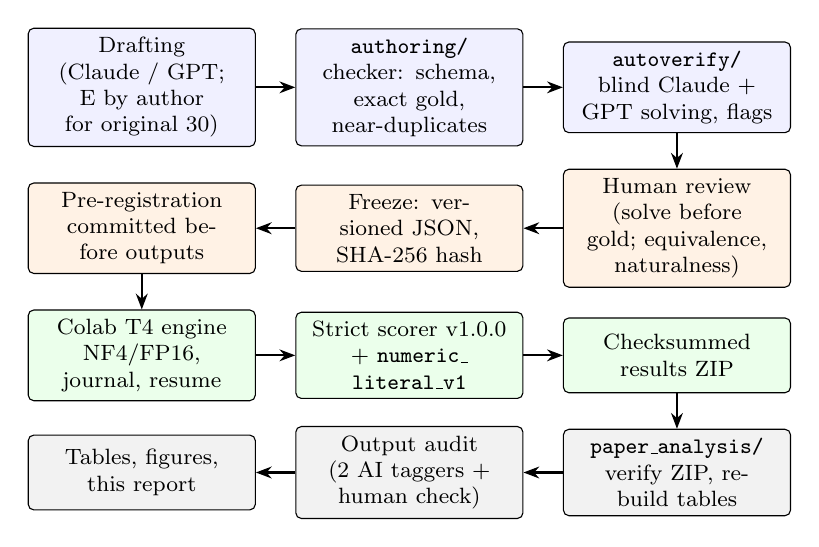
\begin{tikzpicture}[
  node distance=0.45cm and 0.5cm,
  box/.style={draw, rounded corners=2pt, align=center, font=\footnotesize, minimum height=0.95cm, text width=2.65cm, fill=#1},
  box/.default={white},
  arr/.style={-{Stealth[length=2mm]}, thick}]
\node[box=blue!6] (author) {Drafting\\(Claude / GPT; E by author for original 30)};
\node[box=blue!6, right=of author] (check) {\texttt{authoring/}\\checker: schema, exact gold, near-duplicates};
\node[box=blue!6, right=of check] (blind) {\texttt{autoverify/}\\blind Claude + GPT solving, flags};
\node[box=orange!10, below=of blind] (human) {Human review\\(solve before gold; equivalence, naturalness)};
\node[box=orange!10, left=of human] (freeze) {Freeze: versioned JSON, SHA-256 hash};
\node[box=orange!10, left=of freeze] (prereg) {Pre-registration committed before outputs};
\node[box=green!8, below=of prereg] (engine) {Colab T4 engine\\NF4/FP16, journal, resume};
\node[box=green!8, right=of engine] (score) {Strict scorer v1.0.0\\+ \texttt{numeric\_literal\_v1}};
\node[box=green!8, right=of score] (zip) {Checksummed results ZIP};
\node[box=gray!10, below=of zip] (pa) {\texttt{paper\_analysis/}\\verify ZIP, rebuild tables};
\node[box=gray!10, left=of pa] (audit) {Output audit\\(2 AI taggers + human check)};
\node[box=gray!10, left=of audit] (report) {Tables, figures, this report};
\draw[arr] (author) -- (check);
\draw[arr] (check) -- (blind);
\draw[arr] (blind) -- (human);
\draw[arr] (human) -- (freeze);
\draw[arr] (freeze) -- (prereg);
\draw[arr] (prereg) -- (engine);
\draw[arr] (engine) -- (score);
\draw[arr] (score) -- (zip);
\draw[arr] (zip) -- (pa);
\draw[arr] (pa) -- (audit);
\draw[arr] (audit) -- (report);
\end{tikzpicture}
\caption{Pipeline from drafting to reported tables. Blue: dataset construction; orange: human gate and freeze; green: inference and scoring on Colab; grey: analysis.}
\label{fig:pipeline}
\end{figure}

\section{Evaluation engine and Colab notebooks}

The evaluation engine (\texttt{test1\_pilot/hinglish\_pilot/}) has modules for data validation (\texttt{data.py}), the run loop (\texttt{engine.py}), the Hugging Face backend (\texttt{hf\_backend.py}), reporting (\texttt{report.py}) and the scorer (\texttt{scorer\_v1.py}, a byte-for-byte copy of the original \texttt{pilot/scripts/scorer.py}). A builder script embeds all of this, together with fixtures and documentation, into a single self-contained notebook, so a team member only uploads one \texttt{.ipynb} file to Colab and chooses \emph{Run all}. Separate notebooks were built for each cohort and model (\texttt{colab\_notebooks/pilot\_b\_eval/}, \texttt{pilot\_original\_eval/}) and for model screening (\texttt{model\_screening/}). A Pilot-B notebook takes about 25--35 minutes on a T4.

\paragraph{Modes.} The engine has four modes, each with its own validation gate:
\begin{itemize}[nosep]
\item \texttt{demo}: a fake backend with synthetic fixtures, for software checks only;
\item \texttt{reviewed}: 30 families with two reviews and adjudication;
\item \texttt{pilot\_b}: 1--200 families with single-reviewer attestation and split role \texttt{PILOT\_B\_EVAL} (D035);
\item \texttt{pilot\_adjudicated}: the original-cohort mode (D036), with \texttt{judgment\_source} recorded per reviewer form (D037).
\end{itemize}
Research modes reject the fake backend, DRAFT status and the wrong split role. Every run's outputs carry a label naming its evidence type (for example ``PILOT-B EVALUATION --- single-reviewer frozen data'').

\paragraph{Inference recipe.} The engine loads the model and tokenizer at immutable revisions resolved on first load, using NF4 with double quantization and FP16 compute on a single CUDA device, with the SDPA math kernel and no adapters. It uses greedy non-thinking decoding with generation seed 11 and deterministic per-item seeds, a 1,024 new-token cap, a total context preflight cap of 2,048 tokens and batch size 1. The verified stack is torch 2.11.0+cu130, transformers 4.51.3 and bitsandbytes 0.50.2. Before scored generation, every prompt is tokenized and checked, so that no question is truncated. Silent changes to the cap or precision, CPU offloading, thinking mode and model substitution are all forbidden.

\paragraph{Journal and resume.} Colab sessions disconnect. Each generation attempt is journaled \emph{before} it starts and committed as an atomic JSON file. On resume, the engine reuses frozen input snapshots and immutable revisions. It refuses to continue if the data, configuration, code, backend facts or package environment have changed, and it skips successful generations even when they are wrong, refused, malformed or truncated. At most one infrastructure retry is allowed, with unchanged settings and a preserved record. Out-of-memory errors stop the run instead of being retried. A lock file prevents two writers in one run directory, and a stale lock can be recovered only by an explicit setting. Headline accuracy is suppressed until every required output is complete.

\paragraph{Checksummed export.} The results ZIP contains manifests, exact input snapshots and prompts, attempt records, automatic predictions, per-family comparisons, metrics, errors, an audit CSV and a \texttt{checksums.sha256} file covering every member. Export uses a fixed allow-list of files and rejects common credential and e-mail patterns. CSV cells that begin with spreadsheet formula characters receive a protective apostrophe (a bug in this guard, which also prefixed empty strings, was fixed before any pilot run; D022). Manual audit overlays are stored as separate versioned revisions and never overwrite automatic scores.

\section{Scoring}

\paragraph{Strict scorer v1.0.0 (primary).} The scorer finds exactly one \texttt{FINAL:} line, which must be the last non-blank line, and parses an exact rational value. It then validates the unit text against the family's canonical unit, aliases and conversions. Dimensionless answers must carry no suffix. Missing, duplicate or non-terminal FINAL lines, unsupported values, invalid units, refusals and truncation are all scored wrong, with a recorded \texttt{invalid\_reason}.

\paragraph{\texttt{numeric\_literal\_v1} (secondary).} Implemented in \texttt{secondary\_analysis/numeric\_endpoint.py} and adopted under D018, this endpoint never consults gold during extraction. It requires exactly one FINAL marker at the start of a line (bold variants allowed), never recovers an answer from other lines and fails truncated outputs. Its grammar accepts an optional one-letter assignment (\texttt{x =}), an optional currency prefix (\rs, INR, Rs., Rs), a scalar optionally wrapped in \texttt{**}, \texttt{\$} or \verb|\boxed{}|, and an optional word suffix. The literal value is compared with gold exactly, with no unit conversion. The grammar has no rule for a currency symbol \emph{after} the number; Chapter~\ref{ch:results} shows the consequence.

\paragraph{CMI.} The same package implements a Code-Mixing Index (CMI\_v1) over token tags that a single bilingual human corrects from heuristic pre-tags. Its output is labelled as heuristic and single-annotator.

\section{Analysis and verification tools}

\paragraph{\texttt{paper\_analysis/}.} This standard-library tool turns results ZIPs into Markdown and LaTeX tables, a combined per-rendering CSV and figures. It adds no new scoring. It treats ZIPs as untrusted: they are read into memory, never extracted or executed, and absolute or \texttt{..} paths, symlinks and encrypted, duplicate or oversized members are rejected. Every checksum entry must match, every member must be listed, and attempt record hashes and snapshot hashes are verified against the run manifest. It recomputes accuracy, Wilson intervals and the paired bootstrap with the same formulas and random-number order as the engine, checks them against the stored \texttt{metrics.json}, and exits with code 3 on any mismatch. Runs are never pooled. All six cohort runs reproduced the stored metrics exactly.

\paragraph{\texttt{autoverify/}.} \label{sec:autoverify}This toolkit makes blind solver tasks and compares the answers. \texttt{make\_solver\_tasks.py} writes one shuffled task file per solver containing only four whitelisted fields (family ID, rendering ID, form, text), so gold, equations and metadata never reach a solver. \texttt{compare.py} joins outputs by rendering ID and rejects malformed, duplicate or unknown rows. It flags gold mismatches, solver disagreement, cross-form quantity or target mismatches, ambiguity notes and missing outputs. It then writes a review sheet listing all flagged families plus a seeded random 20\% of the unflagged ones, with the gold column placed last so it can be hidden until the reviewer has assessed the question. Automated checks never assign ACCEPT.

\paragraph{\texttt{authoring/}.} \label{sec:authoring}The authoring kit has a family template, a guide and \texttt{check\_family.py}. The checker validates structure and the gold schema and evaluates the reference equation with a safe AST evaluator in exact fractions. It also finds duplicate texts and flags character 5-gram Jaccard similarity of 0.5 or more against the pilot drafts and the format fixtures, reporting IDs only and never printing pilot gold. The guide's independence rules forbid adapting public benchmarks, forbid derivatives of the pilot and fixtures, treat numeric siblings as the same family, require operation-word balancing for C, and forbid authors from reviewing their own families.

\paragraph{Training preparation (\texttt{t4\_smoke/}).} Model-free code for the planned training smoke test builds completion-only labels. It masks the rendered generation prompt, including Qwen3's empty think block, and supervises the English solution plus the end token. It also asserts that the target token IDs are identical across E, R and C. No training has been run.

\section{Testing}

All suites were re-run for this report on 26 October 2026 with Python 3.12, without GPU dependencies. Table~\ref{tab:tests} lists the current counts; every test passed. On 15 October the corresponding counts were 22 pipeline, 38 secondary-analysis, 3 scorer and 4 training-protocol tests, and the suites have grown since.

\begin{table}[t]
\centering\small
\caption{Software test suites (re-run 26 October 2026; all passing).}
\label{tab:tests}
\begin{tabularx}{\linewidth}{@{}lLr@{}}
\toprule
Suite & What it covers & Tests\\
\midrule
\texttt{test1\_pilot/tests} & Engine: malformed review/split/gold rejection, exact numeric/unit scoring, invalid and truncated outputs, paired bootstrap and discordance, bounded retries, interruption, lost in-flight generation, stale locks, incompatible resumes, journal corruption, overlays, secret detection & 23\\
\texttt{secondary\_analysis/tests} & \texttt{numeric\_literal\_v1} grammar, CMI, secondary report, notebook freshness & 64\\
\texttt{autoverify/tests} & Task whitelisting, seeded shuffles, output validation, flags, review-sheet sampling & 23\\
\texttt{t4\_smoke} & Training-protocol validation and completion-only labels & 21\\
\texttt{paper\_analysis/tests} & Safe ZIP reading, checksum verification, table consistency & 17\\
\texttt{authoring/tests} & Family checker: schema, equation exactness, near-duplicates & 10\\
\texttt{pilot/scripts} & Original exact scorer (including 60 balanced answer cases) & 3\\
\midrule
Total & & 161\\
\bottomrule
\end{tabularx}
\end{table}

Beyond unit tests, the notebook was validated with nbformat, executed end-to-end in a fresh Jupyter kernel in demo mode, and its exports passed checksum verification. A real-GPU smoke run on a Colab T4 (Qwen3-4B; T4 with 14.56~GiB reported device memory) completed six short generations with no infrastructure errors or truncation. Model load took about 224.75~s (possibly including download), and per-generation reserved memory peaked at about 4.19~GiB. That smoke run's original 0/6 automatic score exposed a fixture error, a blank gold unit on a count question, and the strict suffix rule on fractions. The fixture was repaired in a new demo version and the original scores were preserved. This was the first sign of the format problem studied in Chapter~\ref{ch:dev}.

\section{Real-browser test of the review forms}

The original pilot's reviewers used offline HTML forms (stage~1 solving, stage~2 rating; Appendix~\ref{app:forms}). On 20 October 2026 a script drove headless Google Chrome (via puppeteer-core) through \emph{copies} of the R01 stage-1, R01 stage-2 and R02 stage-2 forms using artificial answers; the distributed packets were not modified. All 14 checks passed with no page JavaScript errors:
\begin{itemize}[nosep]
\item stage~1 loads 90 renderings and shows no gold;
\item partial progress downloads and resumes by import;
\item completing all solves with timestamps and the attestation exports correctly;
\item stage~2 blocks saving before import and rejects an unfinished stage~1;
\item stage~2 accepts a finished stage~1, keeps its answers unchanged and records its SHA-256;
\item ratings for all 90 rows export;
\item R02's stage~2 rejects an R01 file.
\end{itemize}
The test also produced three usability notes. The stage-1 import message (``Imported answers are read-only in stage2'') may confuse reviewers. Progress and final downloads share one filename, so the browser renames repeats and reviewers must return the last file. The packet's C definition is the original clause-based one. The form itself never writes an AI-prefill field, which is how the R01 stage-2 provenance marker was later recognized as external to the form (Section~\ref{sec:review}).

%======================================================================
\chapter{Development Findings on Excluded Fixtures}
\label{ch:dev}
%======================================================================

\evid{development evidence only. All results in this chapter come from 36 AI-authored, unreviewed fixture prompts (12 families $\times$ E/R/C, \texttt{FMT2}), permanently excluded from both cohorts and from all later training and test data. With 12 prompts per form, every rate is a rough indication, not an estimate.}

Before spending the one-shot cohort runs, the project ran the 12 fixture families through the identical pipeline on a Colab T4. The aim was to find protocol problems on data that would never be used as evidence.

\section{The format confound and the prompt v1$\to$v2 change}

The original instruction (\texttt{test1-english-final-v1}) asked for \texttt{FINAL: <number or fraction> <unit when applicable>}. Under it, 10 of 36 Qwen3-4B outputs were strict-invalid, all with \texttt{invalid\_unit} (Table~\ref{tab:fmt2}). In 8 outputs, spread roughly equally across forms, the model appended a unit word to a dimensionless answer: \texttt{8 unitless}, \texttt{24 unit.}, \texttt{8 unit (no unit specified, so just the number)} and \texttt{7/27 positions.}. In one R output (\texttt{109 moti.}) the model echoed the question's Hindi noun, which was not among that fixture's aliases. Since the original pilot has 6 dimensionless families out of 30, the v1 prompt would have failed many correct answers on them in every form. There were no missing, multiple or non-terminal FINAL lines and no refusals.

\begin{table}[t]
\centering\small
\caption{Qwen3-4B on the 36 excluded FMT2 fixture prompts under prompt v1 and v2 (development evidence; counts of 12 per form).}
\label{tab:fmt2}
\begin{tabular}{@{}llccccc@{}}
\toprule
Prompt & Form & \makecell{Strict\\correct} & \makecell{Numeric\\match} & \makecell{Strict\\invalid} & \makecell{Devanagari\\in output} & \makecell{Median\\output tokens}\\
\midrule
\multirow{3}{*}{v1} & E & 9 & 12 & 3 & 0 & 82\\
 & R & 7 & 10 & 4 & 8 & 107\\
 & C & 9 & 11 & 3 & 0 & 86\\
\midrule
\multirow{3}{*}{v2} & E & 12 & 12 & 0 & 0 & --\\
 & R & 10 & 10 & 0 & 0 & --\\
 & C & 12 & 12 & 0 & 0 & --\\
\bottomrule
\end{tabular}
\end{table}

Decision D020 replaced the instruction with \texttt{test1-english-final-v2} (Appendix~\ref{app:prompt}): explain in English even when the question is not in English; after FINAL, write a unit in English only if the answer has one, and nothing after a pure number. The v1 text is kept in the code as \texttt{INSTRUCTION\_V1}, and the scorer was unchanged. Under v2, Qwen3-4B produced 0/36 invalid outputs. Dimensionless answers became bare (\texttt{FINAL: 8}) and units became English (\texttt{330 rupees}, \texttt{59 minutes}). The strict and numeric endpoints agreed on all 36 outputs, and strict-correct counts were 12/10/12.

The fixtures also changed between the two runs. One ambiguous R rendering was repaired (FMT2-001-R, where a fee could be read as per-plate), and the alias \emph{moti} was added; the fixture version went from 0.1.0 to 0.2.0. The 10$\to$0 change is therefore a development comparison, not an isolated prompt effect. The revision was made once, disclosed and versioned. Prompt iteration on the fixtures then stopped, and the prompt was frozen before any cohort generation.

\section{Devanagari drift}

Under v1, 8 of 12 R outputs contained Devanagari script despite the instruction to explain in English, and about 10 of 12 contained Romanized-Hindi prose; E had 0/12 and C had about 2/12 with Romanized prose only. Under v2, Devanagari fell to 0/12 R outputs, and a heuristic marker found Romanized-Hindi prose in 1 of 12. The detector is heuristic, not a validated language tag. This drift does not affect either scoring endpoint. It does show that output-language following degrades on Romanized-Hindi input, which made the English-compliance audit of Chapter~\ref{ch:results} essential.

\section{Repeated \emph{bhaag}/\emph{bhinn} misreadings}

Under v2, Qwen3-4B's only two errors were R items. In FMT2-005-R, \emph{bhaag dekar bhinn likho} (``divide, write as a fraction'') was answered as a difference. In FMT2-006-R, \emph{kitna bhinn istemaal hua} (``what fraction was used'') received the remaining count (20) under both v1 and v2, and Llama-3.2-3B later gave the same 20. Claude, an AI assistant, judged both renderings correct; no independent bilingual check was made. \emph{Bhinn} means both ``fraction'' and ``different'', even in Devanagari. With $n=2$ unreviewed items, these errors are \emph{consistent with} operation-word misreading but do not establish it. They motivated the lexicon and the keep/switch design of Pilot-B (Section~\ref{sec:lexicon}), both fixed before any cohort output and tested in Chapter~\ref{ch:results}.

\section{Seven-model format screening and the inclusion rule}

Decision D028 screened more unchanged models on the same 36 prompts under the frozen v2 prompt, recipe and scorer. Its pre-declared rule was that a model joins the cohort evaluations only if at most 3/36 fixture outputs are strict-invalid, with no per-model prompt or scorer tuning. Table~\ref{tab:screen} summarizes the screen.

\begin{table}[t]
\centering\small
\caption{Format screening on the excluded fixtures (prompt v2; strict-invalid of 36; strict correct of 12 per form). Development evidence. $^\dagger$primary; $^\times$excluded.}
\label{tab:screen}
\begin{tabularx}{\linewidth}{@{}lccLl@{}}
\toprule
Model & Invalid & E/R/C & Dominant failure & Decision\\
\midrule
Qwen3-4B$^\dagger$ & 0 & 12/10/12 & 2 R operation-word misreadings & Primary\\
Qwen3-8B & 0 & 12/12/12 & none (1 R output with Devanagari) & Included (D030)\\
Llama-3.2-3B-Instruct & 2 & 12/9/9 & value errors in R and C; 1 truncation, 1 missing FINAL & Included (D032)\\
Qwen3-1.7B$^\times$ & 36 & 0/0/0 & instruction echo on the FINAL line & Excluded (D029)\\
Phi-4-mini-instruct$^\times$ & 14 & 6/4/11 & inline FINAL; R repetition to the token cap & Excluded (D025)\\
Granite-3.3-2B-instruct$^\times$ & 36 & 0/0/0 & commentary after FINAL & Excluded (D026)\\
Gemma-3-4B-it$^\times$ & -- & -- & no outputs (CUDA error under FP16) & Excluded (D031)\\
\bottomrule
\end{tabularx}
\end{table}

Phi-4-mini and Granite were excluded before the $\le$3/36 rule was formalized; both exceed it. Phi-4-mini's failures show why such a screen is needed. In 7 outputs it wrote the FINAL marker inline at the end of a paragraph, which both endpoints reject, and 6 of its 12 R outputs collapsed into repetition at the 1,024-token cap, in four cases echoing the Hindi question 17--40 times. Its apparent C~$>$~E ordering (11/12 vs 6/12) is therefore a formatting artifact. Granite commented on the unit instruction after the answer (e.g.\ \texttt{FINAL: 24, (units: none)}), so most of its numerically right values were rejected. Qwen3-1.7B copied the instruction's wording onto the FINAL line. Gemma-3-4B loaded but every generation failed with a CUDA error under the frozen FP16 recipe; running it would have required a model-specific recipe change, which D028 does not allow.

Two lessons follow. First, within Qwen3, instruction following broke before mathematics did: 36/36 invalid at 1.7B against 0/36 at 4B and 8B. Second, one frozen prompt and scorer cannot simply be applied across model families. Without a compliance check on excluded data, a multi-model comparison would mostly measure formatting. The cohort evaluations therefore use three backbones: Qwen3-4B (primary), Qwen3-8B (within-family scaling) and Llama-3.2-3B (cross-family). The latter two are secondary and descriptive.

%======================================================================
\chapter{Results}
\label{ch:results}
%======================================================================

\evid{cohort results under pre-registered plans. Pilot-B (70 families, single-reviewer data, insertional C) is primary. The original cohort (24 families, clause-based C) is a descriptive replication whose plan was written with Pilot-B results known. The two cohorts are never pooled. Each backbone ran once per cohort and completed every rendering (210/210 and 72/72), with all checksums verified; the tables reproduce the stored scores exactly.}

\section{Pilot-B: accuracy by form}

Table~\ref{tab:pilotb_acc} gives strict accuracy per form for the three backbones, and Figure~\ref{fig:pilotb} plots it. R is the lowest-scoring form for every backbone.

\begin{table}[t]
\centering\small
\caption{Pilot-B strict accuracy (70 families per form): correct count, accuracy (\%) and 95\% Wilson interval, and strict-invalid outputs (truncations in parentheses). No refusals occurred.}
\label{tab:pilotb_acc}
\setlength{\tabcolsep}{4pt}\footnotesize
\begin{tabular}{@{}lccc@{}}
\toprule
Backbone & E & R & C\\
\midrule
Qwen3-4B (primary) & 66/70 \enspace 94.3 [86.2, 97.8] & 60/70 \enspace 85.7 [75.7, 92.1] & 66/70 \enspace 94.3 [86.2, 97.8]\\
\quad invalid & 3 & 2 & 1\\
Qwen3-8B & 69/70 \enspace 98.6 [92.3, 99.7] & 64/70 \enspace 91.4 [82.5, 96.0] & 69/70 \enspace 98.6 [92.3, 99.7]\\
\quad invalid & 1 & 1 & 0\\
Llama-3.2-3B & 66/70 \enspace 94.3 [86.2, 97.8] & 40/70 \enspace 57.1 [45.5, 68.1] & 49/70 \enspace 70.0 [58.5, 79.5]\\
\quad invalid & 1 & 6 (5) & 4 (2)\\
\bottomrule
\end{tabular}
\end{table}

\begin{figure}[t]
\centering
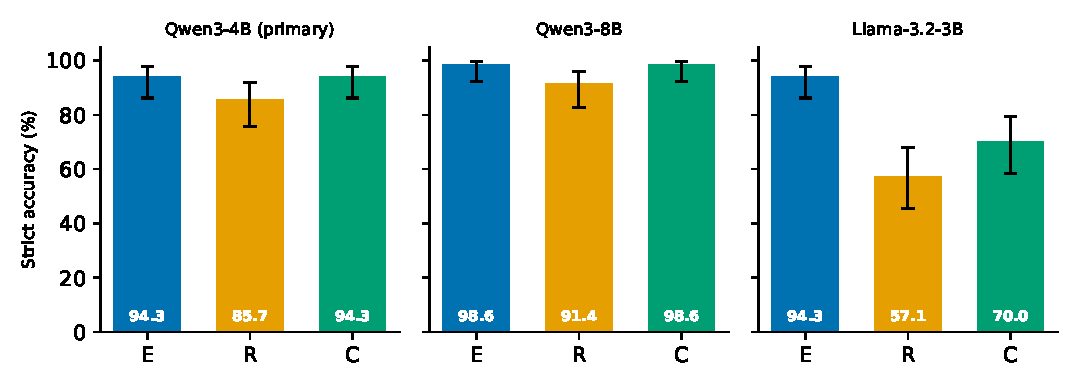
\includegraphics[width=\linewidth]{figures/accuracy_by_form.pdf}
\caption{Pilot-B strict accuracy by form with 95\% Wilson intervals (70 families per bar).}
\label{fig:pilotb}
\end{figure}

\section{Pilot-B: paired differences}

Because the three forms share their families, the relevant comparison is paired (Table~\ref{tab:pilotb_diff}).

\begin{table}[t]
\centering\small
\caption{Pilot-B paired family differences (percentage points) with 95\% intervals from 10,000 family-bootstrap resamples (seed 101). In parentheses: discordant families correct only in the first / only in the second form.}
\label{tab:pilotb_diff}
\setlength{\tabcolsep}{2.5pt}\footnotesize
\begin{tabular}{@{}lccc@{}}
\toprule
Backbone & E$-$R & E$-$C & R$-$C\\
\midrule
Qwen3-4B & $+$8.6 [$-$1.4, $+$18.6] (9/3) & 0.0 [$-$7.1, $+$7.1] (3/3) & $-$8.6 [$-$15.7, $-$1.4] (1/7)\\
Qwen3-8B & $+$7.1 [0.0, $+$14.3] (6/1) & 0.0 [$-$4.3, $+$4.3] (1/1) & $-$7.1 [$-$14.3, 0.0] (1/6)\\
Llama-3.2-3B & $+$37.1 [$+$24.3, $+$50.0] (28/2) & $+$24.3 [$+$11.4, $+$37.1] (21/4) & $-$12.9 [$-$27.1, $+$1.4] (10/19)\\
\bottomrule
\end{tabular}
\end{table}

\begin{enumerate}[nosep]
\item \textbf{R is the weakest form for all three backbones.} The deficit depends strongly on the model: it is modest for Qwen (8.6 and 7.1 points, with intervals crossing or touching zero) and large for Llama (37.1 points, with an interval well above zero).
\item \textbf{E and C have equal observed aggregate accuracy for both Qwen models} (E$-$C $=$ 0.0). This is not itemwise identity, since the discordances are 3/3 and 1/1, and it is not an equivalence test. C exceeds R, and for Qwen3-4B the R$-$C interval excludes zero (C better in 7 families, R better in 1).
\item \textbf{For Llama, C lies between E and R}, 24.3 points below E.
\item \textbf{Scale within Qwen.} Going from 4B to 8B raises R from 85.7\% to 91.4\% and E/C from 94.3\% to 98.6\%. The E$-$R gap moves only from 8.6 to 7.1 points.
\end{enumerate}

\section{Pilot-B: operation-word strata}

Table~\ref{tab:strata} gives the pre-registered descriptive split by whether C keeps R's Hindi operation word, switches it to English, or R has none, and Figure~\ref{fig:strata} plots the R column. R accuracy is similar across strata for every model, so the R deficit is \emph{not concentrated} in items with \emph{bhaag}/\emph{bhinn}-type vocabulary. The misreading hypothesis suggested by the two development errors is not supported at this scale. Many Llama R errors are arithmetic slips on simple items; for example, in PB017 ($1200 - 3\times265 = 405$) Llama answered 435.

\begin{table}[t]
\centering\small
\caption{Pilot-B strict accuracy by pre-registered operation-word stratum (descriptive; counts and percentages only).}
\label{tab:strata}
\begin{tabular}{@{}llcccc@{}}
\toprule
Backbone & Stratum & Families & E & R & C\\
\midrule
\multirow{3}{*}{Qwen3-4B} & C keeps & 18 & 18 (100\%) & 16 (89\%) & 17 (94\%)\\
 & C switches & 17 & 17 (100\%) & 14 (82\%) & 17 (100\%)\\
 & none & 35 & 31 (89\%) & 30 (86\%) & 32 (91\%)\\
\midrule
\multirow{3}{*}{Qwen3-8B} & C keeps & 18 & 18 (100\%) & 17 (94\%) & 17 (94\%)\\
 & C switches & 17 & 17 (100\%) & 16 (94\%) & 17 (100\%)\\
 & none & 35 & 34 (97\%) & 31 (89\%) & 35 (100\%)\\
\midrule
\multirow{3}{*}{Llama-3.2-3B} & C keeps & 18 & 18 (100\%) & 12 (67\%) & 13 (72\%)\\
 & C switches & 17 & 16 (94\%) & 10 (59\%) & 11 (65\%)\\
 & none & 35 & 32 (91\%) & 18 (51\%) & 25 (71\%)\\
\bottomrule
\end{tabular}
\end{table}

\begin{figure}[t]
\centering
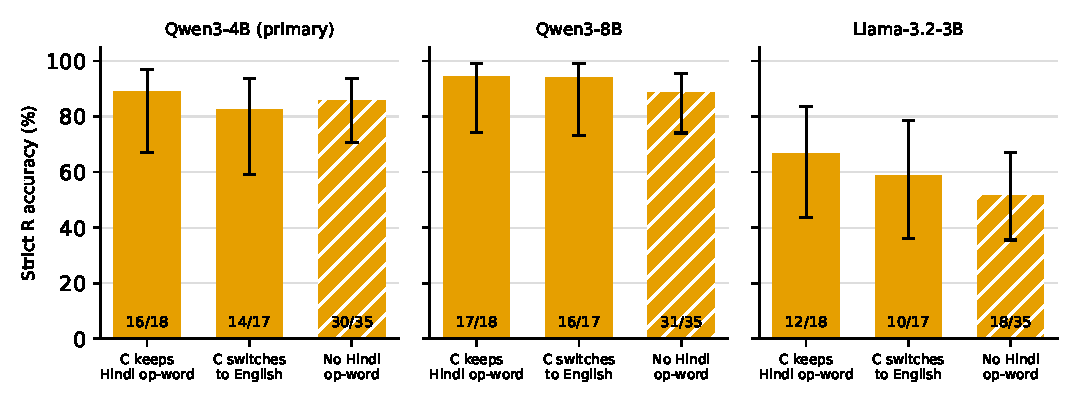
\includegraphics[width=\linewidth]{figures/pilotb_r_by_stratum.pdf}
\caption{Pilot-B strict R accuracy by operation-word stratum with 95\% Wilson intervals; bar labels give correct/families. Regenerated from \texttt{results/pilot\_b/*/per\_rendering.csv} with the stratum rule of \texttt{results/pilot\_b/strata.py}.}
\label{fig:strata}
\end{figure}

\section{Pilot-B: residual format effects}

\paragraph{Strict-invalid outputs.} All six of Qwen3-4B's strict-invalid outputs are \texttt{invalid\_unit}. Three of its four E failures are numerically correct answers given with English unit phrases outside the aliases (\texttt{11 years old}, \texttt{13 years old}, \texttt{4 bags of cement}). One C failure is an unlisted spelling (\texttt{300 rupye}), the form-dependent alias penalty anticipated before the pilot. Together these cost Qwen3-4B four strict points. Qwen3-8B's only strict-invalid E output is \texttt{11 years old.} (PB065-E). For Llama, the stored invalid reasons (from \texttt{per\_rendering.csv}) are: E, one \texttt{invalid\_numeric\_grouping}; R, five truncations and one \texttt{invalid\_unit}; C, two truncations, one \texttt{missing\_final} and one \texttt{invalid\_numeric\_grouping}.

\paragraph{Endpoint agreement.} The numeric endpoint agrees with strict scoring on all 210 Llama Pilot-B renderings. This does not rule out formatting failures that both endpoints reject: Llama had 11 strict-invalid outputs, 7 of them truncated.

\paragraph{The trailing-\rs\ gap in the secondary endpoint.} For Qwen, the frozen numeric grammar does not accept a \emph{trailing} rupee symbol (\texttt{FINAL: 1575 \rs}), which the strict scorer accepts as a unit. This accounts for every strict-correct/numeric-fail case: 30 for Qwen3-4B and 36 for Qwen3-8B. As a result, \texttt{numeric\_literal\_v1} falls \emph{below} strict for both Qwen models (Table~\ref{tab:numeric}). The gap lies in the endpoint's specification, not in the models. It is reported as pre-registered and the endpoint is not changed. A post-hoc sensitivity check, not pre-registered, that allows the trailing symbol restores agreement with strict on all 36 Qwen3-8B cases; the only other Qwen3-8B disagreement is PB065-E.

\begin{table}[t]
\centering\small
\caption{Pilot-B secondary endpoint \texttt{numeric\_literal\_v1} beside strict accuracy (\%). The Qwen shortfall is the trailing-\rs\ specification gap.}
\label{tab:numeric}
\begin{tabular}{@{}lcccccc@{}}
\toprule
 & \multicolumn{3}{c}{Strict} & \multicolumn{3}{c}{Numeric}\\
\cmidrule(lr){2-4}\cmidrule(lr){5-7}
Backbone & E & R & C & E & R & C\\
\midrule
Qwen3-4B & 94.3 & 85.7 & 94.3 & 72.9 & 82.9 & 82.9\\
Qwen3-8B & 98.6 & 91.4 & 98.6 & 84.3 & 74.3 & 80.0\\
Llama-3.2-3B & 94.3 & 57.1 & 70.0 & 94.3 & 57.1 & 70.0\\
\bottomrule
\end{tabular}
\end{table}

\section{Pilot-B: resources}

Table~\ref{tab:resources} gives the stored median token counts and latencies (pre-registered endpoint~6). R prompts are longer than E for every model (123 vs 109 input tokens for Qwen, 138 vs 124 for Llama). The input count covers the whole prompt, including the chat template and the fixed instruction. Llama's R outputs are also longer. These are correlates, not causes.

\begin{table}[t]
\centering\small
\caption{Pilot-B median input tokens, output tokens and generation latency (s) by form (70 renderings each; latency excludes model load and tokenization).}
\label{tab:resources}
\begin{tabular}{@{}lccccccccc@{}}
\toprule
 & \multicolumn{3}{c}{Input tokens} & \multicolumn{3}{c}{Output tokens} & \multicolumn{3}{c}{Latency (s)}\\
\cmidrule(lr){2-4}\cmidrule(lr){5-7}\cmidrule(lr){8-10}
Backbone & E & R & C & E & R & C & E & R & C\\
\midrule
Qwen3-4B & 109 & 123 & 119 & 104 & 98.5 & 93.5 & 9.59 & 9.26 & 8.65\\
Qwen3-8B & 109 & 123 & 119 & 72.5 & 73.5 & 72.5 & 7.33 & 7.32 & 7.40\\
Llama-3.2-3B & 124 & 138 & 134.5 & 99 & 119.5 & 96.5 & 5.95 & 7.14 & 5.75\\
\bottomrule
\end{tabular}
\end{table}

\section{Pilot-B: output audit of the primary model}

\paragraph{Method.} Two AI models, Claude and GPT, pre-tagged all 210 Qwen3-4B Pilot-B outputs under written audit instructions, each blind to the other's tags. Each output received an error category, the first applicable in a pre-registered order, and an English-compliance tag. The taggers agreed on the category for 206/210 outputs (Cohen's $\kappa = 0.94$) and on English compliance for 208/210 ($\kappa = 0.96$). A human then checked the 4 disagreement rows and 20 seeded random agreed rows (seed 101), with the taggers anonymized as A and B. The human label agreed with tagger A on 22/24 and with tagger B on 21/24. The final label is the human label where checked (24 outputs) and the agreed AI label otherwise (186 outputs). The audit is therefore an \emph{AI pre-tag, human-checked on disagreements and a sample}. One human label, ``ambiguous'' (PB033-R, flagged as an ambiguous question), is mapped to \emph{unresolved}. This is an audit of model outputs, not of the dataset.

\begin{table}[t]
\centering\small
\caption{Primary audit category per Qwen3-4B Pilot-B output (70 per form) and English-compliant explanations.}
\label{tab:audit}
\begin{tabular}{@{}lrrr@{}}
\toprule
Category & E & R & C\\
\midrule
no\_error & 66 & 47 & 56\\
format\_only & 3 & 2 & 1\\
language\_drift & 0 & 13 & 10\\
wrong\_relation\_operation & 1 & 4 & 2\\
misread\_quantity & 0 & 2 & 0\\
arithmetic\_slip & 0 & 1 & 1\\
unresolved & 0 & 1 & 0\\
\midrule
English-compliant explanation & 70 & 53 & 59\\
\bottomrule
\end{tabular}
\end{table}

\paragraph{Findings.} Of Qwen3-4B's 18 strict failures, 6 are format-only. The substantive errors concentrate in R: 8, against 1 in E and 3 in C. English explanations fell from 70/70 on E to 53/70 on R and 59/70 on C (Table~\ref{tab:audit}). The \emph{language\_drift} rows are strict-correct outputs (with \emph{no\_error} they sum to the strict-correct counts 66/60/66) whose explanation drifted away from English, so instruction following erodes on R and C even when the answer is right.

\paragraph{Exploratory (Llama; not pre-registered).} A heuristic count found that Llama explained 60/70 R and 27/70 C outputs in Romanized-Hindi prose (E: 0/70; no Devanagari). On C, Hindi-prose explanations were correct 13/27 (48\%) against 36/43 (84\%) for English explanations; on R, 35/60 against 5/10. This association is observational and confounded with item difficulty, since harder items may both trigger Hindi explanations and cause errors.

\section{Original cohort results}

Tables~\ref{tab:orig_acc} and~\ref{tab:orig_diff} and Figure~\ref{fig:orig} report the 24-family original cohort. All runs completed (72/72) with zero strict-invalid outputs, and the numeric endpoint agrees with strict scoring on all 72 renderings for each model.

\begin{table}[t]
\centering\small
\caption{Original cohort strict accuracy (24 families per form) with 95\% Wilson intervals. No strict-invalid outputs.}
\label{tab:orig_acc}
\setlength{\tabcolsep}{4pt}\footnotesize
\begin{tabular}{@{}lccc@{}}
\toprule
Backbone & E & R & C\\
\midrule
Qwen3-4B (primary) & 24/24 \enspace 100.0 [86.2, 100.0] & 22/24 \enspace 91.7 [74.2, 97.7] & 24/24 \enspace 100.0 [86.2, 100.0]\\
Qwen3-8B & 24/24 \enspace 100.0 [86.2, 100.0] & 23/24 \enspace 95.8 [79.8, 99.3] & 24/24 \enspace 100.0 [86.2, 100.0]\\
Llama-3.2-3B & 21/24 \enspace 87.5 [69.0, 95.7] & 15/24 \enspace 62.5 [42.7, 78.8] & 22/24 \enspace 91.7 [74.2, 97.7]\\
\bottomrule
\end{tabular}
\end{table}

\begin{table}[t]
\centering\small
\caption{Original cohort paired differences (pp) with 95\% family-bootstrap intervals (10,000 resamples, seed 101) and discordant counts. Zero-width intervals at ceiling are not evidence of equivalence.}
\label{tab:orig_diff}
\setlength{\tabcolsep}{4pt}\footnotesize
\begin{tabular}{@{}lccc@{}}
\toprule
Backbone & E$-$R & E$-$C & R$-$C\\
\midrule
Qwen3-4B & $+$8.3 [0.0, $+$20.8] (2/0) & 0.0 [0.0, 0.0] (0/0) & $-$8.3 [$-$20.8, 0.0] (0/2)\\
Qwen3-8B & $+$4.2 [0.0, $+$12.5] (1/0) & 0.0 [0.0, 0.0] (0/0) & $-$4.2 [$-$12.5, 0.0] (0/1)\\
Llama-3.2-3B & $+$25.0 [$+$4.2, $+$45.8] (7/1) & $-$4.2 [$-$16.7, $+$8.3] (1/2) & $-$29.2 [$-$45.8, $-$12.5] (0/7)\\
\bottomrule
\end{tabular}
\end{table}

\begin{figure}[t]
\centering
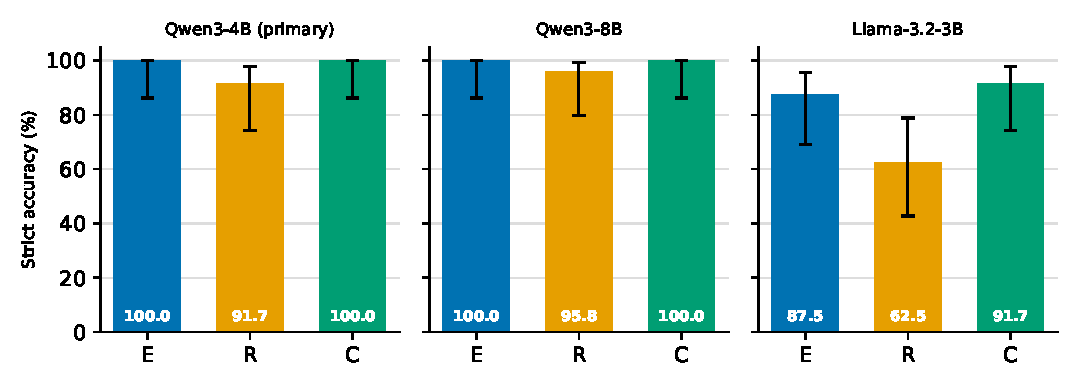
\includegraphics[width=\linewidth]{figures/original_cohort_accuracy.pdf}
\caption{Original cohort strict accuracy by form with 95\% Wilson intervals (24 families per bar). Regenerated from \texttt{results/pilot\_original/*/per\_rendering.csv}.}
\label{fig:orig}
\end{figure}

\paragraph{Individual errors.} Qwen3-4B made two R errors. In PIL001-R it answered 41 against gold 31, treating \emph{Riya se 5 kam} (``5 fewer than Riya'') as addition; this is an isolated operation-word (\emph{kam}) misreading. In PIL028-R it answered 50/9~cm, a wrong value. Qwen3-8B's only error is PIL025-R (answered 3, a wrong value). Llama made 14 errors, 9 of them in R; PIL007 is wrong in all three forms (answered 12), so it is not a language effect.

\section{Descriptive cross-cohort comparison}

Table~\ref{tab:cross} is the one pre-specified side-by-side comparison. It reports each cohort's own within-cohort estimates; there is no pooling, no cross-cohort test, no combined interval and no cross-cohort pairing. The cohorts differ in families, sample size, topic and operation-word composition, review process and C definition, so no difference between them can be attributed to any single factor.

\begin{table}[t]
\centering\small
\caption{Pre-specified descriptive comparison of the two cohorts (never pooled). Strict accuracy (\%) and paired differences (pp), each computed within its own cohort.}
\label{tab:cross}
\begin{tabular}{@{}llrcccccc@{}}
\toprule
Backbone & Cohort & $N$ & E & R & C & E$-$R & E$-$C & R$-$C\\
\midrule
\multirow{2}{*}{Qwen3-4B} & Pilot-B & 70 & 94.3 & 85.7 & 94.3 & $+$8.6 & 0.0 & $-$8.6\\
 & Original & 24 & 100.0 & 91.7 & 100.0 & $+$8.3 & 0.0 & $-$8.3\\
\midrule
\multirow{2}{*}{Qwen3-8B} & Pilot-B & 70 & 98.6 & 91.4 & 98.6 & $+$7.1 & 0.0 & $-$7.1\\
 & Original & 24 & 100.0 & 95.8 & 100.0 & $+$4.2 & 0.0 & $-$4.2\\
\midrule
\multirow{2}{*}{Llama-3.2-3B} & Pilot-B & 70 & 94.3 & 57.1 & 70.0 & $+$37.1 & $+$24.3 & $-$12.9\\
 & Original & 24 & 87.5 & 62.5 & 91.7 & $+$25.0 & $-$4.2 & $-$29.2\\
\bottomrule
\end{tabular}
\end{table}

The direction replicates for every model: R is the lowest form in both cohorts. Qwen is near ceiling in the original cohort (E $=$ C $=$ 100\%). Llama's R deficit appears in both cohorts (E$-$R $+$37.1 and $+$25.0 points). C's position for Llama differs: well below E in Pilot-B, but at E's level in the original cohort. C's position relative to E is therefore model- and cohort-dependent.

%======================================================================
\chapter{Discussion}
\label{ch:discussion}
%======================================================================

\section{Romanized Hindi, not code-mixing, is the hard case here}

In both cohorts and for all three backbones, the Hinglish rendering was never the lowest-scoring form; Romanized Hindi was. For both Qwen models, Hinglish matched English in observed aggregate accuracy in both cohorts. Popular intuition often treats mixing two languages in one sentence as the difficult part of Hinglish. These results suggest that, for these models and items, the difficulty sits more with the Hindi-dominant Roman-script form. Insertional Hinglish keeps many English content words (\emph{ratio}, \emph{add}, \emph{total}), and these may anchor the model's understanding.

Some care is needed in stating this. ``E $=$ C'' here is equality of two observed proportions on 70 or 24 families. It is not itemwise identity (there are 3/3 discordant families for Qwen3-4B in Pilot-B) and not an equivalence test with a margin. For Llama in Pilot-B, C is 24.3 points below E, so ``code-mixing is harmless'' is not a supported general claim. Because all three forms are in Latin script, the design cannot separate a romanization penalty from a Hindi-vocabulary or register effect (Chapter~\ref{ch:limits}).

\section{Model dependence}

The size of the R deficit varies roughly four- to fivefold across backbones (7--9 points for Qwen, 37 for Llama in Pilot-B). Llama is as good as Qwen3-4B on English (94.3\% each) but far worse on R. A benchmark result on one model family is therefore a weak guide to another, and the development screen showed that even \emph{whether} a model can be scored under a given format depends on the model.

\section{Scale}

Within Qwen3, the 8B model improves every form, but the R deficit remains (8.6 $\to$ 7.1 points in Pilot-B). Scale helps overall accuracy more than it closes the language-form gap. In the development screen the most dramatic scale effect was on instruction following, not mathematics: 1.7B could not follow the answer format at all, while 4B and 8B followed it perfectly. With one model family per size, this is an observation, not a scaling law.

\section{The operation-word null result}

The development study produced a vivid hypothesis: R errors come from ambiguous Hindi operation words such as \emph{bhinn} (fraction/different). The keep/switch design of Pilot-B was built to test it, and the strata show no concentration of R errors in families containing such words. R accuracy is similar whether C keeps the word, C switches it, or there is no such word at all. The audit points the same way: Qwen3-4B's eight substantive R errors are spread across wrong relations, misread quantities, an arithmetic slip and one unresolved case, and Llama's R errors include plain arithmetic slips. One clear operation-word misreading did occur in the original cohort (\emph{Riya se 5 kam} read as addition), so such misreadings happen. They do not, however, explain most of the gap. With strata of 17--35 families this is a descriptive null, not proof that vocabulary plays no role.

This null result illustrates why the protocol separated development evidence from cohort evidence. Two striking fixture errors suggested a mechanism, and a balanced, pre-registered design did not support it.

\section{Instruction-following erosion}

A second, quieter effect runs through the data: models increasingly ignore the instruction to explain in English as the input moves away from English. Under prompt v1, 8 of 12 R fixture explanations were in Devanagari. Under v2, in Pilot-B, Qwen3-4B's English compliance fell from 70/70 (E) to 53/70 (R) and 59/70 (C). Llama explained 60 of 70 R outputs in Romanized-Hindi prose. The model often reasons in the language it was addressed in, even when told otherwise. This matters for applications that need consistent output language, and it matters for evaluation, because a scorer or extractor tuned to English text can silently penalize such outputs.

\section{Comparison with prior work}

The direction of the main result matches CodeMixTax~\citep{sthanika-2026-codemix}, which reports Romanized Hindi below Romanized Hinglish across models on translated GSM8K. The gaps there are larger (for example 90.26/66.18/40.63 for Gemma-3-4B on E/Romanized-Hinglish/Romanized-Hindi). That study uses scheme-style romanization of machine-translated items, while this project uses newly drafted, human-reviewed renderings in natural spelling, with a strict scorer checked on excluded data. A replication of the direction under these different conditions makes the ordering more credible. Differences in magnitude cannot be attributed to any one factor, because the models, items and protocols all differ.

The scoring findings echo \citet{peter-etal-2026-mind}: evaluation details can create apparent language effects. Here, a single phrase in the answer-format instruction produced form-dependent scoring failures on development data. The pre-registered secondary endpoint's trailing-\rs\ gap shows that even a carefully specified extractor can have blind spots, and the unlisted English unit phrases (\texttt{11 years old}) show that strict scoring has a cost too. Reporting both endpoints side by side, unchanged, lets readers see these effects instead of having them silently absorbed into accuracy.

Sarvam-M~\citep{sarvam-2025-sarvamm} and the health-triage study of \citet{khullar-etal-2026-script} report degradation on Romanized Indic input relative to native script; this project cannot test that contrast because it has no Devanagari arm. CodeMixBench~\citep{yang-chai-2025-codemixbench} reports lower accuracy on mixed-script Hindi--English GSM8K than on English, which is consistent with Llama's Pilot-B E$-$C gap but not with Qwen's E $=$ C. This is a reminder that ``code-mixed'' covers several scripts and registers.

%======================================================================
\chapter{Limitations and Ethics}
\label{ch:limits}
%======================================================================

\section{Limitations}

\paragraph{Sample size.} With 70 and 24 families, intervals are wide and the operation-word strata (17--35 families) are sparse and descriptive. Model-free power calculations showed that detecting a 5-point paired difference needs hundreds of families. The original cohort is near ceiling for Qwen, and its analysis plan was written after Pilot-B results were known.

\paragraph{Single-reviewer data.} Pilot-B, FINAL\_TEST and the lexicon were each reviewed by one bilingual reviewer, who is a team member. TRAIN and DEV received sample-based review of 45 families. The original cohort had two independent human solvers but one human language reviewer plus the adjudicator. Naturalness judgments reflect the register of very few speakers. A second-annotator sample is planned (D027).

\paragraph{AI-drafted items.} Most renderings were drafted by an LLM, and the items may share LLM drafting styles. Claude both drafted and blind-solved Pilot-B. The GPT/Claude repair-rate contrast (68/100 vs 13/70) is confounded with split, prompt and review timing.

\paragraph{Review-integrity issues and how they were handled.} The original pilot's review surfaced several problems. Each was handled by excluding the affected evidence, not by repairing it after the fact.
\begin{itemize}[nosep]
\item Earlier review rounds turned out not to be independent. They were discarded and archived as unused, as were later edited copies of returned files.
\item The two returned re-reviews of the five repaired families were byte-identical, so they cannot count as independent re-review. Those five families were excluded from the cohort.
\item One reviewer's official stage-2 file carried an AI-prefill marker on 70 of 90 rows, a field that the review form does not write. Those judgments were excluded from all human-review and agreement claims, and the cohort's language review is described as one human plus the adjudicator (D037).
\item The draft metadata labelled the author-written English statements as AI drafts. The author's correction is recorded without altering the frozen files (D038).
\end{itemize}
All exclusions were decided before any model output on the cohort, and the amended plan was committed first.

\paragraph{Different C definitions.} The original cohort uses the clause-based C and Pilot-B the insertional C, which prevents a pooled C estimate. The original 30 drafts also have unbalanced operation words (27/30 R vs 10/30 C).

\paragraph{One model family per size.} The three backbones are two Qwen3 sizes and one Llama model. Scale and family are not crossed, and the format screen excluded four of seven screened models whose formatting the scorer does not accept. The results are conditional on models that can follow the format.

\paragraph{No native-script control.} There is no Devanagari arm, so an E$-$R gap mixes script, language, register and spelling. The pattern C $\approx$ E with R $<$ E points to Hindi vocabulary or register rather than mixing, but does not identify the cause. Each R rendering is also only one of many possible spellings.

\paragraph{Contamination.} The items are new, but the models' pretraining data cannot be audited.

\paragraph{Hardware: T4 and FP16.} All runs use 4-bit NF4 weights, FP16 compute, greedy decoding and no thinking mode on a free T4, which lacks bf16. The results are conditional on this configuration. Gemma-3-4B could not run under FP16 at all. No cross-hardware bitwise reproducibility is claimed.

\paragraph{Residual format effects and thin development evidence.} Strict scoring still penalizes some correct answers (unlisted English unit phrases, the spelling \emph{rupye}), and the secondary endpoint has the trailing-\rs\ gap; both are reported, not corrected. The prompt was revised after seeing outputs on 12 unreviewed fixtures. This is disclosed, and no cohort item was used to design the prompt.

\paragraph{Audit.} The output audit rests on two AI taggers with a human check of disagreements and a 20-row sample, not a full human audit, and it covers only the primary model on Pilot-B.

\paragraph{No training yet.} RQ2 and RQ3 are untested.

\section{Ethics}

\paragraph{Consent and credit.} Reviewers received a consent note covering the task, data use and release, and all reviewers consented to release of the data under CC BY 4.0. Reviewers will be credited according to their stated preferences; the adjudicator declined credit. Real identities are kept out of shared ledgers, and reviewers appear only under pseudonyms (R01, R02, A01).

\paragraph{Data.} The items are invented everyday word problems with invented first names, and an automated scan found no contact details. Romanized Hindi varies by region and register, and these renderings reflect few speakers. FINAL\_TEST stays unreleased until the confirmatory evaluation, to protect it from contamination.

\paragraph{Licences.} Data are released under CC BY 4.0 (\texttt{DATA\_LICENSE.md}) and code under the MIT licence (\texttt{LICENSE}), with ``the project authors'' as copyright holder (D034). The student confirmed that DTU has no specific licence requirement.

\section{AI-assistance disclosure}
\label{sec:aidisclosure}

AI assistants were used extensively, and this section states how.
\begin{enumerate}[nosep]
\item \textbf{AI-drafted items.} Renderings were drafted by an LLM: Claude for Pilot-B and TRAIN, and GPT for FINAL\_TEST and DEV. For the original pilot, the English statements were written by the author, and R and C were translated by an LLM (OpenAI GPT via Codex). All families were then checked against code-computed gold and reviewed by humans, and the AI-drafted sets were also verified blind by two LLM solvers.
\item \textbf{AI-assisted human review.} Humans made every acceptance decision. Some lexicon entries and some text edits were drafted by AI before reviewers confirmed them. In the original cohort, one reviewer's AI-prefilled, unverified stage-2 judgments were excluded.
\item \textbf{AI-assisted audit.} The output audit used two AI pre-taggers with a human check.
\item \textbf{Writing, coding and decisions.} AI assistants helped write the evaluation and analysis code, the research notes, the paper draft and this report. Under the student's explicit delegation (D017), they also recorded protocol decisions in the decision log, where each one is labelled as an AI decision under delegation. The student reviewed this work and takes responsibility for it.
\end{enumerate}
Systems used: Claude Opus 5.5 (Anthropic); GPT-6 Astra and GPT-6.1 Sol (OpenAI, via the Codex CLI).

%======================================================================
\chapter{Conclusion and Future Work}
\label{ch:conclusion}
%======================================================================

\section{Conclusion}

With the mathematics held fixed, three small open models were least accurate on Romanized Hindi in two separately reviewed, pre-registered cohorts, by a strongly model-specific amount (about 7--9 points for Qwen, 25--37 for Llama). Both Qwen models had equal observed aggregate accuracy on English and Hinglish. The R errors were not concentrated in items with Hindi operation words, and instruction following eroded on non-English input. On excluded data, a single phrase in the answer-format instruction produced form-dependent scoring failures, and format compliance varied sharply across models. The methodological lesson is that answer formats and scorers must be checked on excluded data before any language comparison is run. The phase also delivered a reproducible pipeline with 161 passing tests, and 300 frozen Phase-2 families ready for the training study.

\section{Phase 2: the training study}

\paragraph{Design.} The essential comparison (D001) is three fine-tuning arms on matched mathematical content with identical English solution targets and matched exposure:
\begin{itemize}[nosep]
\item \textbf{E+E}: English questions only;
\item \textbf{E+R}: English plus Romanized-Hindi questions;
\item \textbf{E+C}: English plus Hinglish questions.
\end{itemize}
Training uses the frozen TRAIN split (160 families), with DEV (40 families) for development checks. A single confirmatory evaluation then runs on the untouched FINAL\_TEST (100 families), together with an English-retention check, to answer RQ2 and RQ3. Matching exposure does not necessarily match input tokens or runtime, so both will be measured per arm.

\paragraph{Recipe (proposed, not yet approved).} The proposal is QLoRA on Qwen3-4B: LoRA rank 16 and alpha 32 on all seven linear projections (33,030,144 trainable parameters), microbatch 1 with 16-step accumulation, a 1,024-token sequence cap, completion-only loss, NF4 with double quantization, FP16 compute and gradient checkpointing. The illustrative budget is three arms $\times$ three seeds $\times$ 256 updates $=$ 2,304 updates. These values, together with the proposed $+$5-point useful-gain and $-$2-point English-retention margins, are discussion proposals that are not yet approved (D015). They must be fixed before any training outcome is seen. Desk estimates put peak memory at about 5.5--7.5~GB against about 14.5~GiB usable, and time at about 8--55~s per update, so 2,304 updates would take about 5--35 GPU-hours before overhead. Time is the main risk.

\paragraph{Feasibility gates (D021).} The smoke test will first try the stack already verified for inference: torch 2.11.0+cu130, transformers 4.51.3, bitsandbytes 0.50.2 and PEFT 0.15.2. It will use a project-owned training loop, not TRL, with self-built completion-only labels that mask the prompt, including the empty think block, and supervise the English solution plus \texttt{<|im\_end|>}. The target token IDs must be identical across E/R/C. The go/no-go thresholds were fixed before any measurement:
\begin{itemize}[nosep]
\item median $\le$56~s per update: stay on Colab;
\item 56--150~s: move to Kaggle 2$\times$T4;
\item $>$150~s: fall back to Qwen3-1.7B.
\end{itemize}
The fallback stack is the older pinned stack in a fresh runtime, with inference re-run. Every arm and seed must use the same GPU model, software stack, recipe and update count.

\section{Timeline to May 2027}

\begin{table}[h]
\centering\small
\caption{Plan for the remainder of the project.}
\label{tab:timeline}
\begin{tabularx}{\linewidth}{@{}lL@{}}
\toprule
Period & Milestone\\
\midrule
Nov 2026 & Minor evaluation. Completed: original-cohort runs and analysis; output audit of Pilot-B (Qwen3-4B). EACL 2027 SRW mentorship draft (6 Nov).\\
Dec 2026 -- Jan 2027 & Training feasibility smoke test on T4 (completion-only loss, memory, checkpoint reload) under the D021 gates; second-annotator sample on Pilot-B and FINAL\_TEST; SRW submission (15 Dec) and notification (5 Jan).\\
Feb -- Mar 2027 & E+E / E+R / E+C fine-tuning with paired seeds on the frozen TRAIN/DEV; one confirmatory evaluation on the untouched FINAL\_TEST, plus English retention.\\
Apr 2027 & Analysis, thesis and training-paper draft.\\
May 2027 & Final submission.\\
\bottomrule
\end{tabularx}
\end{table}

\section{Publication plan}

Under decision D023, the pilot findings target the EACL 2027 Student Research Workshop as a 4-page short paper. The optional mentorship draft is due on 6 November 2026 and direct submission on 15 December 2026; a draft exists in \texttt{paper/latex/main.tex}. The training study targets the ARR May 2027 cycle, whose date is unconfirmed. Co-authorship with the faculty guide is to be discussed with the guide.

\section{Further future work}

Beyond the planned study, the limitations point to clear extensions:
\begin{itemize}[nosep]
\item a reviewed Devanagari arm, to separate script from language;
\item independently authored spelling variants of R;
\item a second independent language reviewer for every cohort;
\item more model families at matched sizes;
\item a full human audit of outputs.
\end{itemize}

%======================================================================
\cleardoublepage
\phantomsection
\addcontentsline{toc}{chapter}{References}
\renewcommand{\bibname}{References}
\bibliographystyle{unsrtnat}
\bibliography{references}

%======================================================================
\appendix

\chapter{Frozen Prompt}
\label{app:prompt}

The system message used for every form and every model (\texttt{test1-english-final-v2}, decision D020) is:

\begin{quote}\small\ttfamily\raggedright
Solve the problem. Give a short explanation in English, even if the question is not in English. End with exactly one line: FINAL: <number or fraction>, followed by its unit in English only if the answer has a unit; write nothing after a pure number or fraction.
\end{quote}

The user message is the question text alone. Decoding is greedy and non-thinking, with a 1,024-token output cap and a fresh context per prompt.

The superseded instruction (\texttt{test1-english-final-v1}, kept in the code as \texttt{INSTRUCTION\_V1}) asked for the final line in the form \texttt{FINAL: <number or fraction> <unit when applicable>}. The phrase ``unit when applicable'' led to unit words on dimensionless answers (Chapter~\ref{ch:dev}).

\chapter{Dataset and Run Hashes}
\label{app:hashes}

All hashes are SHA-256. The dataset hashes were re-computed for this report and match the recorded values.

\begin{table}[h]
\centering\footnotesize
\caption{Frozen dataset files.}
\label{tab:hashes}
\begin{tabularx}{\linewidth}{@{}lrL@{}}
\toprule
File & Families & SHA-256\\
\midrule
\texttt{pilot\_b/pilot\_b\_families.v2.json} & 70 & \hash{e632e5fcc6b050e93d85920d7938fbb229936fa1474095d6c4c4a6517fcf3478}\\
\texttt{phase2/final\_test.v3.json} & 100 & \hash{da89dd9a626e438dffca39e3a74c4c8abc6bb57501495723b87e6ee143f3d46}\\
\texttt{phase2/train\_A.v2.json} & 80 & \hash{b9656a8c41af2a795bce9c131efc6a5efc652df78368d14fb7720fd985883666}\\
\texttt{phase2/train\_B.v2.json} & 80 & \hash{c975fe12459df6160effc5aeb0087f94666ba0b49778c3d827a67bb923ff35bd}\\
\texttt{phase2/dev.v2.json} & 40 & \hash{e741c1652f5b3dcaebc78d9dd9d7c31fdf4417306fbb2f0862149f27f858f28b}\\
\texttt{pilot\_original/cohort\_dataset.json} & 24 & \hash{5c3e8746f0629d1908902658bda2c280aeb388c55e741fb8e612bc49b5d43103}\\
\texttt{pilot\_original/cohort\_splits.json} & -- & \hash{8da8f40eaa01932152032c290f32e20345b7b22092104c0c329d63d0df0067cc}\\
\bottomrule
\end{tabularx}
\end{table}

\noindent The original cohort's canonical-JSON engine digests are \hash{02752d35b6bde18392afb2e02fa3cdc430437801606706a35662bc62fe2ad03a} (dataset) and \hash{8f5996187c291bae21d75fbccb83486ce18bad3b9a13feaaad9fda20a2628433} (splits). Its source draft, \texttt{pilot/annotation\_draft\_v2/coordinator/pilot\_dataset.DRAFT.json}, has hash \hash{9a4434b67941505e9a3679ba6cf0c344f50804230e4fd3591df1f3e192d4711a}.

\begin{table}[h]
\centering\footnotesize
\caption{Returned cohort results ZIPs and pinned model revisions.}
\label{tab:runhashes}
\begin{tabularx}{\linewidth}{@{}llL@{}}
\toprule
Cohort & Model & Returned ZIP SHA-256\\
\midrule
Pilot-B & Qwen3-4B & \hash{7d9274d4af0d4c7599cb68f8353ee6cd695a5d8acd2c22a5facd738f7076e7c5}\\
Pilot-B & Qwen3-8B & \hash{3d1cef58a01116caf7a81f8ace5b641096034735b3e9655267f501ac62455180}\\
Pilot-B & Llama-3.2-3B & \hash{08120040e841b1208f708a83ceec145c02316e2352d1bc8b7a0a29ae39792458}\\
Original & Qwen3-4B & \hash{ff2af2bfd51d3ae301e2c6549f390c8953501c199fe5255ed7a76a19865cab37}\\
Original & Qwen3-8B & \hash{403d7280558d8ba26553d0e07f638650ad87edc08c8b34454f1d0895d1e4509c}\\
Original & Llama-3.2-3B & \hash{5d9b5f657f6cbb147b7adf1b1b84f60414e7fde018d2accb03be21379dd99f31}\\
\midrule
\multicolumn{2}{@{}l}{Model} & Pinned revision\\
\midrule
\multicolumn{2}{@{}l}{\texttt{Qwen/Qwen3-4B}} & \texttt{1cfa9a7208912126459214e8b04321603b3df60c}\\
\multicolumn{2}{@{}l}{\texttt{Qwen/Qwen3-8B}} & \texttt{b968826d9c46dd6066d109eabc6255188de91218}\\
\multicolumn{2}{@{}l}{\texttt{meta-llama/Llama-3.2-3B-Instruct}} & \texttt{0cb88a4f764b7a12671c53f0838cd831a0843b95}\\
\bottomrule
\end{tabularx}
\end{table}

\noindent Development fixture runs (FMT2) have returned ZIP hashes recorded in their \texttt{research/fmt2\_*/\allowbreak README.md} files; for example, the Qwen3-4B prompt-v1 run is \hash{c21741273a1f1c825bc141957a30439b95d567f456e9fc68da0f83e0a004e84f} and the prompt-v2 run is \hash{28794810b54579a6b78f61b36b9354d02eb338cf481dede5869791e7c5cb36d6}.

\chapter{Decision Log Summary}
\label{app:decisions}

The full log is \texttt{docs/DECISIONS.md}. It distinguishes user instructions, human decisions, AI recommendations and AI decisions taken under the student's delegation (D017).

\begin{longtable}{@{}p{1.2cm}p{12.3cm}@{}}
\toprule
ID & Summary\\
\midrule
\endhead
D001 & Essential eventual arms E+E/E+R/E+C, matching content, exposure and full English targets.\\
D002 & Pilot design: unchanged model, 30 families/90 renderings; human acceptance required.\\
D003--D008 & Early process: annotation budget open; review packets distributed; shared-folder coordination; frozen scorer v1 and packets kept unchanged; reviewers not yet done.\\
D009--D011 & Secondary-endpoint specification proposed; currency-prefix and unit-alias handling left to human decision.\\
D012--D014 & One writer at a time; each work cycle must change data/code/results or end with a concrete question; excluded format-test suite proposed.\\
D015 & Training margins (+5pp gain, $-$2pp English), three seeds, 256 updates: discussion proposals, NOT APPROVED.\\
D016--D017 & Minor evaluation November 2026, final May 2027; the student delegated spec-adoption and format-test decisions to Claude; goal is a publishable paper.\\
D018 & Adopted \texttt{numeric\_literal\_v1} as secondary endpoint beside strict v1.0.0; audit taxonomy; CMI\_v1; consent note.\\
D019--D020 & FMT2 format run on excluded fixtures; prompt replaced by \texttt{test1-english-final-v2} before any reviewed generation.\\
D021 & Training-stack plan and go/no-go gates (56~s / 150~s per update).\\
D022 & CSV formula-guard bug fixed before any pilot run.\\
D023 & Publication plan: EACL 2027 SRW (pilot), ARR May 2027 (training).\\
D024--D026 & Phi-4-mini tested and excluded (inline FINAL, R repetition); Granite excluded (commentary after FINAL).\\
D027 & Scale-up: 70-family Pilot-B and 300 Phase-2 families; AI drafting, code gold, Claude/GPT blind solving, human review.\\
D028 & Screen four more models; pre-declared inclusion rule $\le$3/36 strict-invalid.\\
D029--D032 & Qwen3-1.7B excluded; Qwen3-8B included; Gemma-3-4B excluded; Llama-3.2-3B included.\\
D033 & Pilot-B review returned; C redefined as insertional for Pilot-B and Phase 2; R borrowing list extended.\\
D034 & Licences: code MIT, data CC BY 4.0.\\
D035 & Pilot-B evaluated in \texttt{pilot\_b} mode under a plan committed before outputs.\\
D036 & Original cohort = 24 families accepted without repair; excluded PIL010 and five repaired families.\\
D037 & R01's AI-prefilled stage-2 judgments excluded; cohort relabelled (two human solvers; language review R02 + A01); plan amended before outputs.\\
D038 & Provenance correction: original E statements author-written; R/C AI-translated, then human-reviewed.\\
\bottomrule
\end{longtable}

\chapter{The Review Forms}
\label{app:forms}

The original pilot's review used self-contained HTML forms distributed in per-reviewer ZIP packets; reviewers returned the JSON files the forms exported.

\placeholder{Optional: insert a screenshot of the stage-1 and stage-2 forms here, taken from a copy of the packet with artificial answers (never a real reviewer's file).}

\paragraph{Stage 1 (blind solving).} The form presents all 90 renderings in randomized order without any reference answer. For each rendering the reviewer types a numeric answer, and the form records a timestamp. Progress can be downloaded as JSON and resumed by import. When all 90 are solved, the reviewer completes an attestation and downloads \texttt{R01\_stage1\_responses.json} (or R02).

\paragraph{Stage 2 (language review).} This form refuses to save anything before a stage-1 file is imported, and it rejects an unfinished stage-1 file. On import it keeps the stage-1 answers read-only and records the stage-1 file's SHA-256. For each E/R/C triplet the reviewer then rates equivalence, ambiguity, classification (whether R and C meet their definitions) and naturalness, and chooses a disposition. Each reviewer's stage-2 form accepts only that reviewer's own stage-1 file. The form does not write any AI-provenance field.

\paragraph{Adjudication.} The adjudicator's packet, with the reference answers and the decision worksheet, is released only after both independent submissions are collected. The adjudicator records ACCEPT, REVISE or EXCLUDE per family, together with gold and unit decisions. Repaired texts require new versions and an independent re-review.

\paragraph{Pilot-B and Phase 2.} These sets were reviewed through the \texttt{autoverify} review sheet (a CSV with E/R/C texts, flags, \texttt{equivalence\_ok}, naturalness ratings, a decision and notes), with the gold column placed last so it can be hidden until the reviewer has assessed the question.

\chapter{Reproducibility Instructions}
\label{app:repro}

\paragraph{Re-running a cohort evaluation.} Each notebook in \texttt{colab\_notebooks/pilot\_b\_eval/} and \texttt{colab\_notebooks/pilot\_original\_eval/} is self-contained and embeds its frozen data.
\begin{enumerate}[nosep]
\item Open \url{https://colab.research.google.com}, choose File $\to$ Upload notebook, and select, for example, \texttt{PilotB\_Qwen3-4B.ipynb}.
\item Choose Runtime $\to$ Change runtime type $\to$ T4 GPU.
\item For Llama, add a Hugging Face token as a Colab secret, since the model is gated.
\item Choose Runtime $\to$ Run all. A results ZIP downloads at the end. If the session disconnects, rerun with the same run name: the journal resumes and skips completed generations.
\end{enumerate}
Greedy decoding with pinned revisions should reproduce the outputs on the same stack, but no cross-hardware bitwise guarantee is made. A re-run must not overwrite the original returned ZIPs.

\paragraph{Rebuilding the tables.} From the repository root, using only the Python standard library (matplotlib optional, for figures):
\begin{verbatim}
python3 -B -m paper_analysis.build_tables RUN.zip --out NEW_DIR
python3 -B results/pilot_b/strata.py \
    results/pilot_b/qwen3-4b/per_rendering.csv
python3 -B report/figures/make_figures.py
\end{verbatim}
\texttt{build\_tables} verifies every checksum and exits with code 3 if any recomputed value disagrees with the stored metrics. \texttt{--out} must be a new or empty directory.

\paragraph{Re-running the software tests.}
\begin{verbatim}
python3 -B -m unittest discover -s pilot/scripts -p 'test_*.py'
python3 -B -m unittest discover -s t4_smoke -p 'test_*.py'
PYTHONPATH=test1_pilot python3 -B -m unittest discover \
    -s test1_pilot/tests -p 'test_*.py'
python3 -B -m unittest discover -s secondary_analysis/tests
python3 -B -m unittest discover -s paper_analysis/tests
python3 -B -m unittest discover -s autoverify/tests
python3 -B -m unittest discover -s authoring/tests
\end{verbatim}

\paragraph{Blind verification of new families.}
\begin{verbatim}
python3 -B authoring/check_family.py my_families.json
python3 -B autoverify/make_solver_tasks.py families.json \
    --out-dir /tmp/blind-tasks --seed 20261015
python3 -B autoverify/compare.py families.json \
    --claude claude.jsonl --gpt gpt.jsonl --out-dir /tmp/verification
\end{verbatim}

\paragraph{Verifying the frozen data.} \texttt{shasum -a 256} on each file in Table~\ref{tab:hashes} must reproduce the listed hash.


\end{document}
